% This is a modified version of the tufte-latex book example in which the title page and the contents page resemble Tufte's VDQI book, using Kevin Godby's code from this thread at https://groups.google.com/forum/#!topic/tufte-latex/ujdzrktC1BQ.
%
%%%%%%%%%%%%%%%%%%%%%%%%%%%%%%%%%%%%%%%%%%%%%%%%%%%%%%%%%%%%%%%%%%%%%%
% How to use Overleaf: 
%
% You edit the source code here on the left, and the preview on the
% right shows you the result within a few seconds.
%
% Bookmark this page and share the URL with your co-authors. They can
% edit at the same time!
%
% You can upload figures, bibliographies, custom classes and
% styles using the files menu.
%
% If you're new to LaTeX, the wikibook is a great place to start:
% http://en.wikibooks.org/wiki/LaTeX
%
%%%%%%%%%%%%%%%%%%%%%%%%%%%%%%%%%%%%%%%%%%%%%%%%%%%%%%%%%%%%%%%%%%%%%%
%% Unfortunately for the contents to contain
%% the "Parts" lines successfully, hyperref
%% needs to be disabled.
\documentclass[nohyper,nobib]{tufte-book}
\usepackage{nameref}
% \hypersetup{colorlinks}% uncomment this line if you prefer colored hyperlinks (e.g., for onscreen viewing)

% \usepackage{hyphenat}
\usepackage{url}
\usepackage[backend=biber, natbib=true, style=numeric]{biblatex}
\addbibresource{sample-handout.bib}
\usepackage{xargs}
\renewcommandx{\cite}[3][1={0pt},2={}]{\sidenote[][#1]{\fullcite[#2]{#3}}}

%%
% Book metadata
\title{Ginarn}
\date{Version 0.0}
\author[The Ginarn team]{
Sebastien Allegyer,
Rupert Brown,
John Donovan,
Ken Harima,
Aaron Hammond,
Lavanya Kumarappan,
Tao Li,
Ronald Maj,
Bogdan Matviichuk,
Chris Morgan,
Michael Moore,
Simon McClusky,
Thomas Papanikolaou,
Vincent Rooke,
Tzupang Tseng
}
\publisher{Geoscience Australia and Frontier-SI}

%%
% If they're installed, use Bergamo and Chantilly from www.fontsite.com.
% They're clones of Bembo and Gill Sans, respectively.
%\IfFileExists{bergamo.sty}{\usepackage[osf]{bergamo}}{}% Bembo
%\IfFileExists{chantill.sty}{\usepackage{chantill}}{}% Gill Sans

%\usepackage{microtype}

%%
% Just some sample text
\usepackage{lipsum}

%%
% For nicely typeset tabular material
\usepackage{booktabs}

%%
% For graphics / images
\usepackage{graphicx}
\setkeys{Gin}{width=\linewidth,totalheight=\textheight,keepaspectratio}
\graphicspath{{graphics/}}

% The fancyvrb package lets us customize the formatting of verbatim
% environments.  We use a slightly smaller font.
\usepackage{fancyvrb}
\fvset{fontsize=\normalsize}

%%
% Prints argument within hanging parentheses (i.e., parentheses that take
% up no horizontal space).  Useful in tabular environments.
\newcommand{\hangp}[1]{\makebox[0pt][r]{(}#1\makebox[0pt][l]{)}}

%%
% Prints an asterisk that takes up no horizontal space.
% Useful in tabular environments.
\newcommand{\hangstar}{\makebox[0pt][l]{*}}

%%
% Prints a trailing space in a smart way.
\usepackage{xspace}

\usepackage{amsmath}
%%
% Some shortcuts for Tufte's book titles.  The lowercase commands will
% produce the initials of the book title in italics.  The all-caps commands
% will print out the full title of the book in italics.
\newcommand{\vdqi}{\textit{VDQI}\xspace}
\newcommand{\ei}{\textit{EI}\xspace}
\newcommand{\ve}{\textit{VE}\xspace}
\newcommand{\be}{\textit{BE}\xspace}
\newcommand{\VDQI}{\textit{The Visual Display of Quantitative Information}\xspace}
\newcommand{\EI}{\textit{Envisioning Information}\xspace}
\newcommand{\VE}{\textit{Visual Explanations}\xspace}
\newcommand{\BE}{\textit{Beautiful Evidence}\xspace}

\newcommand{\TL}{Tufte-\LaTeX\xspace}

% Prints the month name (e.g., January) and the year (e.g., 2008)
\newcommand{\monthyear}{%
  \ifcase\month\or January\or February\or March\or April\or May\or June\or
  July\or August\or September\or October\or November\or
  December\fi\space\number\year
}


% Prints an epigraph and speaker in sans serif, all-caps type.
\newcommand{\openepigraph}[2]{%
  %\sffamily\fontsize{14}{16}\selectfont
  \begin{fullwidth}
  \sffamily\large
  \begin{doublespace}
  \noindent\allcaps{#1}\\% epigraph
  \noindent\allcaps{#2}% author
  \end{doublespace}
  \end{fullwidth}
}

% Inserts a blank page
\newcommand{\blankpage}{\newpage\hbox{}\thispagestyle{empty}\newpage}

\usepackage{units}

% Typesets the font size, leading, and measure in the form of 10/12x26 pc.
\newcommand{\measure}[3]{#1/#2$\times$\unit[#3]{pc}}

% Macros for typesetting the documentation
\newcommand{\hlred}[1]{\textcolor{Maroon}{#1}}% prints in red
\newcommand{\hangleft}[1]{\makebox[0pt][r]{#1}}
\newcommand{\hairsp}{\hspace{1pt}}% hair space
\newcommand{\hquad}{\hskip0.5em\relax}% half quad space
\newcommand{\TODO}{\textcolor{red}{\bf TODO!}\xspace}
\newcommand{\ie}{\textit{i.\hairsp{}e.}\xspace}
\newcommand{\eg}{\textit{e.\hairsp{}g.}\xspace}
\newcommand{\na}{\quad--}% used in tables for N/A cells
\providecommand{\XeLaTeX}{X\lower.5ex\hbox{\kern-0.15em\reflectbox{E}}\kern-0.1em\LaTeX}
\newcommand{\tXeLaTeX}{\XeLaTeX\index{XeLaTeX@\protect\XeLaTeX}}
% \index{\texttt{\textbackslash xyz}@\hangleft{\texttt{\textbackslash}}\texttt{xyz}}
\newcommand{\tuftebs}{\symbol{'134}}% a backslash in tt type in OT1/T1
\newcommand{\doccmdnoindex}[2][]{\texttt{\tuftebs#2}}% command name -- adds backslash automatically (and doesn't add cmd to the index)
\newcommand{\doccmddef}[2][]{%
  \hlred{\texttt{\tuftebs#2}}\label{cmd:#2}%
  \ifthenelse{\isempty{#1}}%
    {% add the command to the index
      \index{#2 command@\protect\hangleft{\texttt{\tuftebs}}\texttt{#2}}% command name
    }%
    {% add the command and package to the index
      \index{#2 command@\protect\hangleft{\texttt{\tuftebs}}\texttt{#2} (\texttt{#1} package)}% command name
      \index{#1 package@\texttt{#1} package}\index{packages!#1@\texttt{#1}}% package name
    }%
}% command name -- adds backslash automatically
\newcommand{\doccmd}[2][]{%
  \texttt{\tuftebs#2}%
  \ifthenelse{\isempty{#1}}%
    {% add the command to the index
      \index{#2 command@\protect\hangleft{\texttt{\tuftebs}}\texttt{#2}}% command name
    }%
    {% add the command and package to the index
      \index{#2 command@\protect\hangleft{\texttt{\tuftebs}}\texttt{#2} (\texttt{#1} package)}% command name
      \index{#1 package@\texttt{#1} package}\index{packages!#1@\texttt{#1}}% package name
    }%
}% command name -- adds backslash automatically
\newcommand{\docopt}[1]{\ensuremath{\langle}\textrm{\textit{#1}}\ensuremath{\rangle}}% optional command argument
\newcommand{\docarg}[1]{\textrm{\textit{#1}}}% (required) command argument
\newenvironment{docspec}{\begin{quotation}\ttfamily\parskip0pt\parindent0pt\ignorespaces}{\end{quotation}}% command specification environment
\newcommand{\docenv}[1]{\texttt{#1}\index{#1 environment@\texttt{#1} environment}\index{environments!#1@\texttt{#1}}}% environment name
\newcommand{\docenvdef}[1]{\hlred{\texttt{#1}}\label{env:#1}\index{#1 environment@\texttt{#1} environment}\index{environments!#1@\texttt{#1}}}% environment name
\newcommand{\docpkg}[1]{\texttt{#1}\index{#1 package@\texttt{#1} package}\index{packages!#1@\texttt{#1}}}% package name
\newcommand{\doccls}[1]{\texttt{#1}}% document class name
\newcommand{\docclsopt}[1]{\texttt{#1}\index{#1 class option@\texttt{#1} class option}\index{class options!#1@\texttt{#1}}}% document class option name
\newcommand{\docclsoptdef}[1]{\hlred{\texttt{#1}}\label{clsopt:#1}\index{#1 class option@\texttt{#1} class option}\index{class options!#1@\texttt{#1}}}% document class option name defined
\newcommand{\docmsg}[2]{\bigskip\begin{fullwidth}\noindent\ttfamily#1\end{fullwidth}\medskip\par\noindent#2}
\newcommand{\docfilehook}[2]{\texttt{#1}\index{file hooks!#2}\index{#1@\texttt{#1}}}
\newcommand{\doccounter}[1]{\texttt{#1}\index{#1 counter@\texttt{#1} counter}}

% Generates the index
\usepackage{makeidx}
\makeindex

%%%% Kevin Godny's code for title page and contents from https://groups.google.com/forum/#!topic/tufte-latex/ujdzrktC1BQ
\makeatletter
\renewcommand{\maketitlepage}{%
\begingroup%
\setlength{\parindent}{0pt}

{\fontsize{24}{24}\selectfont\textit{\@author}\par}

\vspace{1.75in}{\fontsize{36}{54}\selectfont\@title\par}

\vspace{0.5in}{\fontsize{14}{14}\selectfont\textsf{\smallcaps{\@date}}\par}

\vfill{\fontsize{14}{14}\selectfont\textit{\@publisher}\par}

\thispagestyle{empty}
\endgroup
}
\makeatother

\titlecontents{part}%
    [0pt]% distance from left margin
    {\addvspace{0.25\baselineskip}}% above (global formatting of entry)
    {\allcaps{Part~\thecontentslabel}\allcaps}% before w/ label (label = ``Part I'')
    {\allcaps{Part~\thecontentslabel}\allcaps}% before w/o label
    {}% filler and page (leaders and page num)
    [\vspace*{0.5\baselineskip}]% after

\titlecontents{chapter}%
    [4em]% distance from left margin
    {}% above (global formatting of entry)
    {\contentslabel{2em}\textit}% before w/ label (label = ``Chapter 1'')
    {\hspace{0em}\textit}% before w/o label
    {\qquad\thecontentspage}% filler and page (leaders and page num)
    [\vspace*{0.5\baselineskip}]% after
%%%% End additional code by Kevin Godby

\begin{document}

% Front matter
\frontmatter

% v.2 epigraphs
% \newpage\thispagestyle{empty}
% \openepigraph{%
% The public is more familiar with bad design than good design.
% It is, in effect, conditioned to prefer bad design, 
% because that is what it lives with. 
% The new becomes threatening, the old reassuring.
% }{Paul Rand%, {\itshape Design, Form, and Chaos}
% }
% \vfill
% \openepigraph{%
% A designer knows that he has achieved perfection 
% not when there is nothing left to add, 
% but when there is nothing left to take away.
% }{Antoine de Saint-Exup\'{e}ry}
% \vfill
% \openepigraph{%
% \ldots the designer of a new system must not only be the implementor and the first 
% large-scale user; the designer should also write the first user manual\ldots 
% If I had not participated fully in all these activities, 
% literally hundreds of improvements would never have been made, 
% because I would never have thought of them or perceived 
% why they were important.
% }{Donald E. Knuth}


% r.3 full title page
\maketitle


% v.4 copyright page
\newpage
\begin{fullwidth}
~\vfill
\thispagestyle{empty}
\setlength{\parindent}{0pt}
\setlength{\parskip}{\baselineskip}
Copyright \copyright\ \the\year\ \thanklessauthor

\par\smallcaps{Published by \thanklesspublisher}

\par\smallcaps{tufte-latex.googlecode.com}

\par Licensed under the Apache License, Version 2.0 (the ``License''); you may not
use this file except in compliance with the License. You may obtain a copy
of the License at \url{http://www.apache.org/licenses/LICENSE-2.0}. Unless
required by applicable law or agreed to in writing, software distributed
under the License is distributed on an \smallcaps{``AS IS'' BASIS, WITHOUT
WARRANTIES OR CONDITIONS OF ANY KIND}, either express or implied. See the
License for the specific language governing permissions and limitations
under the License.\index{license}

\par\textit{First printing, \monthyear}
\end{fullwidth}
% r.5 contents
\tableofcontents
%
\chapter{Welcome}
\label{ch:Ginarn}


\newthought{Ginarn} we would like to thank the Wardaman people for the permission in the use of their word Ginarn. 

Ginarn is the fifth-brightest star in the Southern Cross (Epsilon Crucis) . It represents a red dilly-bag filled with special songs of knowledge.
Indigenous Australians often used songs to convey and to pass on knowledge to others, song were also often used as a way to navigate the country.

We hope that you find this software tool kit will convey our understanding on how to process GNSS signals and will also help you to navigate the country!

\newthought{the story} Ginarn was found by Mulugurnden (the crayfish), who brought the red flying foxes from the underworld to the sky. The bats flew up the track of the Milky Way and traded the spiritual song to Guyaru, the Night Owl (the star Sirius). The bats fly through the constellation Scorpius on their way to the Southern Cross, trading songs as they go.

The song informs the people about initiation, which is managed by the stars in Scorpius and related to Larawag (who ensures the appropriate personnel are present for the final stages of the ceremony).

The brownish-red colour of the dilly bag is represented by the colour of Epsilon Crucis, which is an orange giant that lies 228 light years away.
\newthought{This manual} is divided into three major sections: the preliminary matter which gives a quick overview on how to install and use the software with examples. The next part contains the background theory on the models that have been implemented into Ginarn. The back matter contains information about configuration files, and file formats used by the software.
%
\listoffigures
%
\listoftables
%
% r.9 introduction
\cleardoublepage
\part{Overview}
%
\chapter{Introduction to Ginarn GNSS Processing Toolkit}
\label{ch:introduction}
%


Ginarn is a collection of source code that is currently made up two distinct software repositories, the POD \sidenote[][]{https://bitbucket.org/geoscienceaustralia/ pod/wiki/Home} and the PEA\sidenote[][]{https://bitbucket.org/geoscienceaustralia/ pea/wiki/Home}.
Using the POD and PEA together will allow you to estimate your own satellite orbits from a global tracking network.
\newthought{The POD} (precise orbit determination) contains all of the source code needed to determine a GNSS satellite's orbit. You can establish the initial conditions of an orbit from a broadcast ephemeris file, or from an IGS SP3 file. It can then estimate it's own orbital trajectory based upon the models specified in configuration files, and output an SP3 file, or provide a partial files which can then be updated from a tracking network. 



\newthought{The PEA} (parameter estimation algorithm) takes raw observations in RINEX format or in RTCM format, to estimates the parameters you are interested in. You can run it a single user mode, taking in orbit and clocks supplied by real-time streams to SP3 files obtained from the IGS to estimate your own position in static and kinematic mode. 
You can also run the PEA in a network mode, and take in a global network of observations to determine your own orbits and satellite clocks to support your application.

\newthought{The software} is aimed at supporting Australia's implementation of a national positioning infrastructure that supports the objective of 'instantaneous GNSS positoning anywhere, anytime, with the highest possible accuracy and the highest possible integrity.

\newthought{Carrier phase ambiguity}. The underlying signals transmitted by the Global Navigation Satellite Systems (GNSS) can be considered as waves, just like repeating sine waves from high school mathematics. Measurements of these waves are referred to as carrier phase observations, and they are used to provide the precise distance, with mm precision and accuracy, between the orbiting satellites and user’s receiver that are subsequently used to compute position. However, a complicating factor is that carrier phase observations have an ambiguous component where the total whole number of waves, or integer cycles, between the satellite and the user’s receiver cannot be measured, only the fractional part. The unknown number of integer cycles is called the carrier phase ambiguity. Fortunately, the ambiguities can be estimated, and the mathematical and statistical solution to this problem is known as integer ambiguity estimation. While there is a long history of research in this area, which has largely focused on GPS applications, the most optimal solution to this problem when simultaneously combining data from all the GNSS remains unresolved.

\newthought{Atmosphere delay of GNSS signals}. The Earth is surrounded by layers of gases held by Earth's gravity. Signals, such as those transmitted by GNSS, propagated from space are delayed as they pass through the atmosphere. In the troposphere, the region from the Earth’s surface to approximately 20 km altitude, the delay is proportional to temperature, pressure and humidity. The ionosphere, the region from 50-1000 km altitude, causes delay as a function of the frequency of the signal. The composition of both the troposphere and ionosphere vary both in space and time, and this variability currently limits the accuracy, speed and reliability of positioning. But it’s not all bad news, and like a CAT scan in medical science, the new GNSS signals and satellites can potentially be combined to provide a more complete three dimensional picture of the atmospheric delay as a function of time. Models that more completely remove the nuisance atmospheric signals will lead to improved accuracy, speed and reliability of positioning.

\newthought{Precise Point Positioning (PPP) and Real Time Kinematic (RTK)}. Conventional positioning technologies almost exclusively use a technique called Real Time Kinematic (RTK). The RTK technique takes information from nearby Continuously Operating Reference Stations (CORS) to generate corrections for measurements made by users. One of the most important of these is the carrier phase ambiguity correction. The ability to correctly determine carrier phase ambiguities with RTK is determined by many factors, such as the distance between the reference stations and the user and also atmospheric effects. Consequently, RTK relies on relatively dense CORS networks with a typical spacing of 30 to 70 km. An alternative to RTK is Precise Point Positioning (PPP). The PPP technique, rather than directly using measurements from nearby reference stations, uses global satellite orbit and clock information such as that provided by the International GNSS Service. The major advantage of PPP is that it doesn’t require a dense CORS network nearby the user’s location just access to global products. Unfortunately, the PPP technique can have difficulties in resolving carrier phase ambiguities in real time, but additional research focused on greater exploitation of multi-GNSS data and more regional approaches may in the future overcome this limitation.
%
\chapter{Installation}
\label{ch:installation}


\section{To Install} 

In this section we will describe how to install the PEA and POD from source.

\subsection{PEA}


\newthought{Dependencies} the following packages need to be installed with the minimum versions as shown below. This guide will outline the preferred method of installation.

CMAKE  > 3.0 requires openssl-devel to be installed (requires openssl-devel)
YAML   > 0.6
Boost  > 1.70
gcc    > 4.1
Eigen3
Build
To build the PEA Precise Estimation Algorithm...

We suggest using the following directory structure when installing the ACS toolkit. It will be created by following this guide.

%/data/
%└── acs/
%    ├── pea/
%    └── pod/

The following is an example procedure to install the dependencies necessary to run the pea on a base ubuntu linux distribution

Update the base operating system:
\begin{verbatim}
$ sudo apt update
$ sudo apt upgrade
\end{verbatim}
Install base utilities gcc, gfortran, git, openssl, blas, lapack, etc
\begin{verbatim}
$ sudo apt install -y git gobjc gobjc++ gfortran libopenblas-dev openssl curl net-tools openssh-server cmake make \
liblapack-dev gzip vim libssl1.0-dev python3-cartopy python3-scipy python3-matplotlib python3-mpltoolkits.basemap
Create a temporary directory structure to make the dependencies in:
$ sudo mkdir -p /data/tmp
$ cd /data/tmp
\end{verbatim}

\newthought{YAML}
We are using the YAML library to parse the configuration files used to run many of the programs found in this library (https://github.com/jbeder/yaml-cpp). Here is an example of how we have installed the yaml library from source:
\begin{verbatim}
$ cd /data/tmp
$ sudo git clone https://github.com/jbeder/yaml-cpp.git
$ cd yaml-cpp
$ sudo mkdir cmake-build
$ cd cmake-build
$ sudo cmake .. -DCMAKE\_INSTALL\_PREFIX=/usr/local/ -DYAML\_CPP\_BUILD\_TESTS=OFF
$ sudo make install yaml-cpp
$ cd ../..
$ sudo rm -fr yaml-cpp
\end{verbatim}

\newthought{Boost}
We rely on a number of the utilities provided by boost (https://www.boost.org/), such as their time and logging libraries.
\begin{verbatim}

$ cd /data/tmp/
$ sudo wget -c https://dl.bintray.com/boostorg/release/1.73.0/source/boost_1_73_0.tar.gz
$ sudo gunzip boost_1_73_0.tar.gz
$ sudo tar xvf boost_1_73_0.tar
$ cd boost_1_73_0/
$ sudo ./bootstrap.sh
$ sudo ./b2 install
$ cd ..
$ sudo rm -fr boost_1_73_0/ boost_1_73_0.tar

\end{verbatim}

\newthought{Eigen3} is used for performing matrix calculations, and has a very nice API.
\begin{verbatim}
$ cd /data/tmp/
$ sudo git clone https://gitlab.com/libeigen/eigen.git
$ cd eigen
$ sudo mkdir cmake-build
$ cd cmake-build
$ sudo cmake ..
$ sudo make install
$ cd ../..
$ sudo rm -rf eigen
Installing PEA
PEA Executable
$ cd /data/acs/
\end{verbatim}
Clone the repository via https:

\begin{verbatim}
$ git clone https://bitbucket.org/geoscienceaustralia/pea.git
\end{verbatim}
You should now have...

%pea
%├── INSTALL.md
%├── LICENSE.md
%├── README.md
%├── aws/                - for automated builds in aws
%├── config/
%│   ├── Ex00-UnitTest.yaml
%│   ├── Ex01-PPP.yaml
%│   ├── Ex02-Network.yaml
%│   ├── Ex03-Network_Orbits.yaml
%│   ├── Ex04-Ionosphere.yaml
%│   ├── Ex05-Realtime.yaml
%│   ├── iontest_20115w.yaml
%│   └── PPP-iontest.yaml
%├── cpp/
%│   ├── CMakeLists.txt
%│   ├── cmake           - files to help cmake find dependencies
%│   ├── docs            - automatic code documentation configuration
%│   └── src/
%│       ├── 3rdparty/   - see ACKNOWLEDGEMENTS in README.md
%│       ├── common/     - libraries used by the pea
%│       ├── iono/       - routines for ionosphere modelling
%│       ├── pea/        - main for `pea`
%│       └── rtklib/     - subset of modified routines from RTKlib see ACKNOWLEDGEMENTS in README.md
%└── python
%    ├── config
%    ├── README.md
%    └── source
%        ├── download_examples.py
%        ├── install_examples.py
%        └── other helper programs
Prepare a directory to build in, its better practise to keep this separated from the source code.
\begin{verbatim}
$ cd pea/cpp
$ mkdir -p build
$ cd build
\end{verbatim}

Run cmake to find the build dependencies and create the make file:

\begin{verbatim}
$ cmake ..
\end{verbatim}$ 
Now build the pea

\begin{verbatim}
$ cmake --build $PWD --target pea
\end{verbatim}

To change to build location substitute your preferred destination for $PWD , e.g /usr/local/bin

Alternatively to the command above you can make the code in parallel using:
\begin{verbatim}
$ make -j 5 all
\end{verbatim}

where the -j flag controls how many jobs can be run at the same time.

Check to see if you can execute the pea:
\begin{verbatim}
$ ./pea    
\end{verbatim}

and you should see something similar to:
\begin{verbatim}
PEA starting...
Options:
  --help                      Help
  --verbose                   More output
  --quiet                     Less output
  --config arg                Configuration file
  --trace_level arg           Trace level
  --antenna arg               ANTEX file
  --navigation arg            Navigation file
  --sinex arg                 SINEX file
  --sp3file arg               Orbit (SP3) file
  --clkfile arg               Clock (CLK) file
  --dcbfile arg               Code Bias (DCB) file
  --ionfile arg               Ionosphere (IONEX) file
  --podfile arg               Orbits (POD) file
  --blqfile arg               BLQ (Ocean loading) file
  --erpfile arg               ERP file
  --elevation_mask arg        Elevation Mask
  --max_epochs arg            Maximum Epochs
  --epoch_interval arg        Epoch Interval
  --rnx arg                   RINEX station file
  --root_input_dir arg        Directory containg the input data
  --root_output_directory arg Output directory
  --start_epoch arg           Start date/time
  --end_epoch arg             Stop date/time
  --dump-config-only          Dump the configuration and exit
PEA finished
\end{verbatim}

\newthought{The documentation} for the pea can be generated similarly using doxygen if it is installed.

\begin{verbatim}
$ sudo apt-get install doxygen
$ cd pea/cpp/build
$ make doc_doxygen
\end{verbatim}
The docs can then be found at doc\_doxygen/html/index.html

\subsection{POD from source}

%The ACS Version 0.0.1 beta release supports:

%The POD
%Directory Structure
%pod/
%├── LICENSE.md
%├── INSTALL.md
%├── README.md
%├── src/
%├── bin/  (created)
%├── lib/  (created)
%├── config/
%├── tables/
%├── scripts/

Dependencies

The open basic linear algebra library (Openblas.x86\_64,liblas-libs.x86\_64) (You may need to run the command ln -s /usr/lib64/libopenblas.so.3 /usr/lib64/libopenblas.so)
A working C compiler (gcc will do), a working C++ compiler (gcc-g++ will do) and a fortran compiler (we have used gfortran)
Cmake (from cmake.org) at least version 2.8
If the flags set in CMakeLists.txt do not work with your compiler please remove/replace the ones that don't

Build
To build the POD ...
\begin{verbatim}

$ cd pod
$ mkdir build
$ cd build
$ cmake3 .. 
$ make >make.out 2>make.err
$ less make.err (to verify everything was built correctly)
    
\end{verbatim}
You should now have the executables in the bin directory: pod crs2trs brdc2ecef

Test
To test your build of the POD ... - You may not need the ulimit command but we found it necessary

\begin{verbatim}

$ cd ../pod/test
$ ulimit -s unlimited
$ ./sh_test_pod
At the completion of the test run, the sh_test_pod script will return any differences to the standard test resuts
    
\end{verbatim}

Configuration File
The POD Precise Orbit Determination (./bin/pod) uses the configuration file: 
%├── EQM.in (Full force model equation of motion) ├── VEQ.in (For variational equations) ├── POD.in (For all other config)


%\section{From precompiled binaries}
%
%To do..
%
%\include{implementation overview of software}
% block diagram from aaron
%
\include{PEA_Examples}
%
\include{POD_examples}
%
% Start the main matter (normal chapters)
\mainmatter

\part{Background Theory}
\chapter{GNSS Overview}
\label{ch:GNSSOverview}

\section{GPS}

\section{Glonass}

\section{Galileo}

\section{Beidou}

\section{QZSS}

\newthought{The PEA and POD} is designed to do some stuff.
%
\chapter{Observation Modelling}
\label{ch:observation_modelling}

\section{Ionosphere-Free Observations}

\section{Undifferenced - Uncombined}
To do ..
\newthought{The PEA and POD} is designed to do some stuff.

\section{GPS Quarter Cycle}
\begin{fullwidth}
The $L_2$ Civil code (L2C-code) is shifted by a quarter cycle with respect to the P-code. If a receiver is using either the one or the other code to reconstruct the carrier phase measurements, then they will also be shifted by a quarter of a wavelength relative to each other.\\
The noise of phase measurement based on L2C-code is usually lower than the noise of phase observations reconstructed based on p-code. However this is only possible to obtain from satellites that have launched since GPS Block IIR-M was deployed. Older GPS satellites do not provide the L2C-code signal.\\
In RINEX version 2, in order to prevent potential problems in ambiguity resolution some receiver manufactures do correct the phase measurements by 0.25 cycles to keep the phase observations consistent, while others provide the uncorrected phase measurements, an din other cases the user can decide if the correction is applied. Since RINEX version 3.02 the definition has been defined that the phase measurements need to be corrected to have a consistent set of observable that can be introduce for ambiguity resolution.\\
One option to prevent having the quarter cycle issue is to ensure that ambiguities are not resolved between a Block IIR-M or later  with an older satellite.
\end{fullwidth}

\section{Single-satellite and Single-Receiver Observation Combinations}

Linear combinations of the original observations are often applied to eliminate model parameters (eg ionosphere slant delays) or to transform ambiguity parameters (eg widelane transformation). Some of these transformations maintain the information content of the system as they are invertible, but other transformation that are used are do not, and these should be used with caution as the information that contributes to the parameters of interest are lost.\\
%
A large number of different permutations of linear combinations can be formed, with just the dual-frequency legacy signals, this can increases even more as more additional frequencies are available with modernized GNSS signals are deployed. We will only cover the ones used by the PEA in this manual.\\
%
Combining two or more carrier-phase observations into a new signal leads to a different frequency/wavelength. To generalise in the case of a combination for which $\sigma \alpha = 1$, the combined frequency $f_c$ is:
\begin{equation}
f_c = \sigma_{j=1}^n i_j f_j 
\label{eq:comb_freq}
\end{equation}

Remembering that all frequencies for GNSS are derived from a single frequency $f_0$ by multiplication with an integer $k_j$, the individual frequency is obtained from $f_j = j_jf_0$. substituting this into the above equation

$f_c = (\sigma_{j=1}^n i_j k_j) = kf_0$ \label{eq:}

where $k$ is the \emph{lane number}. The corresponding wavelength is:

$\lambda_c = c / kf_0 = \lambda_0 / k$ 

where $\lambda_0$ is the wavelength of the base frequency $f_0$. Since all $i_j$ and $k_j$ are integers, $k$ is also an integer. This parameter uniquely defines the frequency and wavelength of the new signal combination.

With the help of the lane number $k$, the combinations can be categorized into three groups:
\begin{enumerate}
    \item \emph{wide-lane} combination,where the combined wavelength is larger than the largest individual wavelength in the combination.
    \item \emph{intermediate} combinations, for which $\lambda_0$ leas between the largest and shortest individual wavelength.
    \item \emph{narrow-lane} combinations which have a shorter wavelength than the individual signal with the shortest wavelength in the combination.
\end{enumerate}

\newthought{The zero-differenced}, ionosphere free mathematical model for code and phase measurements using dual-frequency can be described by:\\

$ E(P_{r,IF}^S) = \rho_{r}^s + c(dt_{r} - dt^s) + \tau_r^s + c (d_{r,IF} + d_{r,IF}^s) $\label{eq:code_IF_eq}\\

$ E(L_{r,IF}^S) = \rho_{r}^s + c(dt_{r} - dt^s) + \tau_r^s + \lambda_{IF} (z_{r,IF}^s + \delta_{r,IF} - \delta_{IF}^S$\label{eq:phase_IF_eq}\\

with:

$E()$ the expectation notation
$P_{r,IF}^S$ code measurements (m) between satellite $s$ and receiver $r$ for the ionosphere-free measurements;\\
$L_{r,IF}^S$ phase measurements (m)\\
$\rho$ the geometric distance (m)\\
$c$ speed of light (m/s)\\
$dt_r$ receiver clock error (s)\\
$dt^S$ satellite clock error (s)\\
$\tau_r^s $ slant troposphere delay between satellite s and receiver r (m)\\
$dt_{r,IF}$ receiver code bias (s)\\
$dt_{IF}^S$ satellite code bias (s)\\
$\lambda_{IF}$ ionosphere-free wavelength (m)\\
$z_{r,IF}^S$ ionosphere-free ambiguity vector (cycle)\\
$\delta_{r,IF}^S$ receiver ionosphere-free phase bias (cycle)\\
$\delta_{IF}^S$ satellite ionosphere-free phase bias (cycle)\\
%
The ionosphere-free combination will remove the first-order ionosphere delay, both equations are rand deficient and the ambiguity term in eq (2) is not an integer. In order to resolve the ambiguities the linear dependency among the unknown parameters needs to be resolved and the integer property of the ambiguities needs to be recovered. 

\section{Widelane combinations}
The group of wide-lane combinations is especially useful to help with integer ambiguity resolution due to their longer wavelength.

\begin{figure*}[h]
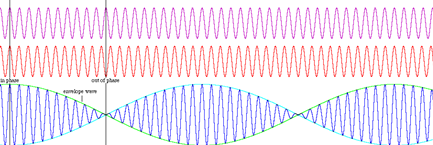
\includegraphics[]{images/widelane.png}
  \caption{Illustration of the linear widelane combinations. Two original frequencies (top and middle) are subtracted to form a longer wavelength observable (bottom)}%
  \label{fig:widelane}%
\end{figure*}



\subsection{Common widelane}
\begin{fullwidth}
To improve ambiguity resolution, often the wide lane linear combination (also called L5 or LW linear combination) is formed from the L1 and L2 carrier phase observables. It is designed to be a geometry-preserving combination using only carrier-phase measurements in the frequencies $f_a$ and $f_b$. By selecting the integer coefficients as $i_A = +1$ and $i_B = -1$, one obtains the WL carrier-phase combination $\phi_{r,WL}^s$ in units of cycles:
\end{fullwidth}
\begin{equation}
\phi_{r,WL}^s = \phi_{r,A}^A - \phi_{r,B}^S = \frac{\psi_{r,A}^s}{\lambda_A} - \frac{\psi{r,B}^s}{\lambda_B} \label{eq:wl_cycles}
\end{equation}

The corresponding wavelength $\lambda_{WL}$ is:
\begin{equation}
\lambda_{WL} = \frac{c}{f_A - f_B} 
    \label{eq:wl_wavelength}
\end{equation}

Multiplication of the two above equations leads to the wide-lane combination $\psi_{r,WL}^s$ in units of meters:
\begin{equation}
\psi_{r,WL}^S = \frac{f_A}{f_A-f_B}\psi_{r,A}^s - \frac{f_B}{f_A-f_B}\psi_{r,B}^s
\end{equation}

\subsection{Melbourne-Wubbena linear combination}
The Melbourne-Wubbena linear combination (Melbourne 1985),(Wubbena 1985) is a linear combination of the L1 and L2 carrier phase plus the P1 and P2 pseudorange. The geometry, troposphere and ionosphere are eliminated by it. The Melbourne-Wubbena linear combination can be represented as:

$
E(L_{r,IF}^S) - \frac{cf_2z_{r,w}^s}{f_1^2 - f_2^2} = \rho_r^s + c(dt_{r,IF} - dt_{IF}^s) + \tau_r^s + \lambda_n z_{r,1}^s + (\lambda_{IF}\delta_{r,IF}$

Since �!,,% comprises of both code and phase measurements, it is reasonable to exclude the lower
elevation measurements to avoid the multipath impacts from the code observation. Normally, with
30 degree elevation cut-off, an averaging of 5 minutes of (4) is good enough to fixing the wide-lane
ambiguities [RD 04]. The rests are the wide-lane phase bias, which can be broadcasted to the user for
user side wide-lane ambiguity resolution. Either choosing a pivot receiver bias or a single-differencing
between two satellites can avoid the linear dependency. 


-doesn't need lambda not as correlated
%
\chapter{Kalman Filtering}
\label{ch:kalman_filter}
%
%
\begin{fullwidth}


The Kalman filter is over 50 years old but is still one of the most important and common data fusion algorithms in use today. 
Named after Rudolf E.Kálmán, the great success of the Kalman filter is due to its small computational requirement, elegant recursive properties, and its status as the optimal estimator for one-dimensional linear systems with Gaussian error statistics. 
Typical uses of the Kalman filter include smoothing noisy data and providing estimates of parameters of interest. 
Kalman filtering is used in a wide range of applications include global positioning system receivers, in control systems, through to the smoothing the output from laptop trackpads, and many more.
%
\end{fullwidth}

\section{Overview of Kalman Filtering}

Kalman filter are typically used to estimate parameters which change with time. 
Parameters with no process noise are called deterministic.
A Kalman filter has measurements $y(t)$, with noise $v(t)$, and a state vector (or a parameter list) which have specified statistical properties.

The observation equation at time t:
\begin{equation}
    y_t = A_t x_t + v_t
\end{equation}

The state transition equation:
\begin{equation}
    x_{t+1} = S_t x_t + w_t
\end{equation}

Covariance matrices
\begin{equation}
    <v_tv_t^T> = V_t , <w_tw_t^T> = W_t 
\end{equation}

The kalman filter processing is broken up into three main steps.
\newthought{Prediction} uses a process noise model to 'predict' the parameters at the next data epoch, subscript is time quantity refrs to, where as the superscript refers to the time of the data:
\begin{equation}
    \hat{x}_{t+1}^t = S_t \hat{x}_t^t
\end{equation}
where, $S_t$ is the state transition matrix
\begin{equation}
    C_{t+1}^t = S_t C_t^t S_t^t + W_t
\end{equation}
where, $w_t$ is the process noise covariance matrix.
The state transition matrix $S$ projects the state vector (parameters) forward to the next epoch.
\begin{itemize}
    \item For random walk $S$ = 1
    \item For rate terms: $S$ is matrix $[1 \delta t][0 1]$
    \item for FOGM: $S$ = $e^{-\delta t \beta}$
    \item For white noise $S$ = 0
\end{itemize}
The second equation projects the covariance matrix of the state vector, $C$, forward in time. Contributions from the state transition and process noise ($W$ matrix). $W$ elements are 0 for deterministic parameters.
%
\newthought{The Kalman gain} is the matrix that allocates the differences between the observation at time t+1 and their predicted value at this time based on the current values of the state vector according to the noise in the measurements and the state vector noise.

\section{Comparison between Weighted Least Squares and Kalman Filtering}

\begin{itemize}
    \item In kalman filtering apriori constraints must be give for all parameters. This is not needed in weighted least squares, but can also be done.
    \item Kalman filters can allow for 0 variance parameters, this cannot be done in WLS, as this requires the inversion of the constraint matrix.
    \item Kalman filter can allow for a method of applying absolute constraints, WLS can only tightly constrain parameters.
    \item Kalman filters are more prone to numerical stability problems, and take longer to run (they have more parameters).
    \item Process noise models can be implemented in WLS, but they are computationally slow.
\end{itemize}

\section{Implementation in the PEA}

\subsection{Observation Weighting}
%
The GNSS observations can be weighted in three different ways in the PEA:
\begin{itemize}
    \item Unity - all observations are assigned the same variance
    \item Elevation Dependent - an elevation dependent function is used to scale the observations, those at higher elevation are given more weight (a smaller standard deviation) than those observed at lower elevation
    \item SNR observations - the Carrier to Noise observations supplied by the receiver are used to determine the observation weight. Generally speaking this is very similar to elevation weighting, but is useful when use observations obtained from a non-geodetic grade receiver/antenna.
\end{itemize}
%
\subsubsection{Unity}

\subsubsection{Elevation Dependent Weighting}

\subsubsection{SNR weighting}


%    // Langley RB (1996) GPS receivers and the observables. In: Kleusberg A, Teunissen PJG (eds) GPS for geodesy.
%    //     Lecture notes in earth sciences, vol 60. Springer, Berlin
%    // Langley, R. B. (1997). "GPS receiver system noise." GPS World, Vol. 8, No. 6, April, pp. 40-45.
%    const double BL = 0.8;      // for code (Hz)
%    const double alpha = 0.5;   // for code (dimensionless)
%    const double BP = 2;        // for phase (Hz)
%    // PI in constants.h

%    //wavelength of the PRN code (in meter)
%    const double P_WL = 29.305;
%    const double CA_WL = 293.05;

%    //wavelength of the carrier phase (in meter)
%    // Teunissen PJG (2017) Carrier-phase integer ambiguity resolution. In: Teunissen PJG, Montenbruck O (eds)
%    //      Handbook of global navigation satellite systems. Springer, Cham, pp 661-685
%    //const double L = lambdas[ft];//lambdas[L1C];// 0.190;


\subsection{Process Noise}

Currently in the PEA we have Gaussian, and random walk process noise models implemented.

The units are in meters, and they are given as $\sigma$ sqrt(variance)

For a random walk process noise, the process noise is incremented at each epoch as $\sqrt{process\_noise}*dt$ where dt is the time step between filter updates.

If you want to allow kinematic processing, then you can increase the process noise e.g.
proc\_noise [0.003]
proc\_noise\_dt: second 

equates to $\frac{0.003}/\sqrt{s}$
\\ 
Or if you wanted highway sppeds 100km/hr = 28 m/s
proc\_noise [28]
proc\_noise\_dt: second
proc\_noise\_model:   Gaussian
or
         proc\_noise\_model:   RandomWalk
or
         proc\_noise\_model:   FOGM 1.0
Where the number after FOGM gives the correlation time B
That way we could keep the same:
            proc\_noise:         [0.01]
            proc\_noise\_dt:      hour

A nice value for using VMF as an apriori value is 0.1mm /sqrt(s)
trop:
            estimated:          true
            sigma:              [0.1]
            proc_noise:         [0.01]
            proc_noise_dt:      hour

\section{Recommended Reading}

\begin{enumerate}
    \item https://ocw.mit.edu/courses/earth-atmospheric-and-planetary-sciences/12-540-principles-of-the-global-positioning-system-spring-2012/lecture-notes/MIT12\_540S12\_lec13.pdf
\end{enumerate}


%
\chapter{Orbit Modelling}
\label{ch:orbit_modelling}


\newthought{POD} is designed to do some stuff.

\section{Gravitational Force Models}

\section{Non-Gravitational Force Models}

\subsection{Solar Radiation Force Models}

\subsection{Cannonball}

\subsection{ECOM I}

\subsection{ECOM II}

\subsection{ECOM C}

\subsection{Box Wing}

\subsection{Antenna Thrust}

\subsection{Albedo}

\section{Transformtation between Celestial and Terrestrial Reference Systems}

The variational equations obtained from the POD need to be transformed into the terrestrial reference frame so that the adjustments can be made in the ECEF frame that the PEA operates in.

\begin{equation}
    [CRS] = Q(t)R(t)W(t)[TRS]
\end{equation}

Where,
$CRS$ is the Celestial Reference System
$TRS$ is the Terrestrial Reference Systems
$Q(t)$ is the Celestial Pole motion (Precession-Nutation) matrix
$R(t)$ is the Earth Rotation matrix
$W(t)$ is the Polar motion matrix
\\
\begin{equation}
Q(t) = 
\begin{bmatrix} 
1-aX^2  & -aXY     & X \\
 -aXY   & 1 - aY^2 & Y \\
 -X     & -Y       & 1-a(X^2+Y^2) 
\end{bmatrix}
\end{equation}
\\
\begin{equation}
R(t) = R_2(-\theta) = 
\begin{bmatrix}
cos \theta & -sin \theta & 0 \\
sin \Theta & cos \theta  & 0 \\
0 & 0 1
\end{bmatrix}
\end{equation}
\\
\begin{equation}
    W(t) = R_z (-s^') R_y(x_p) R_x(y_p)
\end{equation}




%
\chapter{Ionosphere Modelling}
\label{ch:ionosphere_modelling}
\begin{fullwidth}
\newthought{Ionospheric delay} is the most important nuisance parameter on GNSS processing. 
GNSS processing algorithm needs to account for it by estimating, correcting or cancelling its effects. The objective of the project is to develop Ionospheric modelling modules to aid in GNSS data processing. The modules will allow end user position algorithms correct the effect of ionosphere delay. The modules also allow the network processing more effectively estimate the ionospheric delays.\\
%
Two potential ionosphere models have been implemented to date. Both are dual-layer models, each layer containing an ionosphere density map. The maps are represented by spherical cap harmonics in one case and 3rd order b-splines in another. The effectiveness of the maps has been tested using measurements from 60 Australian stations distributed. The geometry free combination of carrier smoothed pseudorange have been used as ionosphere delay measurements. The spherical cap harmonics tested so far can represent the ionospheric delays with an accuracy of about 2-3 TECu, slightly better than the model used for IONEX (single layer, grid based map), but not enough for the 0.2TECu accuracy needed for PPP. The specific parameters (number of layers, map resolution, layer heights and order of the base function) of each model will be refined to improve model accuracy.\\
%
\end{fullwidth}
\section{Ionosphere-Free Observations}

%
\chapter{Ambiguity Resolution}
\label{ch:Ambiguity Resolution}

\begin{fullwidth}
An advantage of the ambiguity fixed solutions is the significantly reduced number of parameters which have to be solved for. A reduction of the normal equation to be inverted is important because usually a duplication of its size leads to over four times longer computing time for the inversion. If many parameters are estimated (orbits, Earth orientation parameters etc.) ambiguity resolution improves also the results of much longer sessions than the traditional daily solution.  
%
Due to the FDMA technology the ambiguity resolution for GLONASS is not a straight forward task, and we have not attempted to implement this into the pea yet.
\end{fullwidth}

There are many methods that can be used to resolve ambiguities, but they mainly consist of two steps:

\begin{enumerate}
    \item The ambiguities are estimates as real numbers (with the other parameters).
    \item Integer values of the ambiguities are resolved using the results of step 1 (the real-value ambiguities and the VCV matrix) employing a number of statistical tests to ensure a reliable estimate.
\end{enumerate}

\begin{fullwidth}
\newthought{Determining a reference or a pivot} is normally done by selecting a station with the most number of observations, however this is not possible to no apriori for a systems that is designed to run in real-time.\\
\end{fullwidth}
%
In the pea we have implemented a number of different ambiguity resolution strategies:
\begin{itemize}
    \item rounding / weighted rounding
    \item bootstrapping
    \item lambda decorelation
    \item BIE
\end{itemize}

\section{rounding algorithm}
The simplest strategy to apply is to round the real-values estimates to the nearest integers, without using any variance co-variance information.

\section{bootstrapping}

The bootstrapping algorithm takes the first ambiguity and rounds its value to the nearest integer. Having obtained the integer value of this first ambiguity, the real-valued estimates of all remaining ambiguities are then corrected by virtue of their correlation with the first ambiguity. Then the second, but now corrected, real-valued ambiguity estimate is rounded to its nearest integer, and the process is then repeated again with both ambiguities held fixed, and the process is continued until all ambiguities are accommodated. Thus the bootstrapped estimator reduces to ’integer rounding’ in case correlations are absent.

\section{lambda}

\section{BIE}


\subsection{Melbourne-Wubbena linear combination}
The Melbourne-Wubbena linear combination (Melbourne 1985),(Wubbena 1985) is a linear combination of the L1 and L2 carrier phase plus the P1 and P2 pseudorange. The geometry, troposphere and ionosphere are eliminated by it. The Melbourne-Wubbena linear combination can be represented as:

$
E(L_{r,IF}^S) - \frac{cf_2z_{r,w}^s}{f_1^2 - f_2^2} = \rho_r^s + c(dt_{r,IF} - dt_{IF}^s) + \tau_r^s + \lambda_n z_{r,1}^s + (\lambda_{IF}\delta_{r,IF}$

Since �!,,% comprises of both code and phase measurements, it is reasonable to exclude the lower
elevation measurements to avoid the multipath impacts from the code observation. Normally, with
30 degree elevation cut-off, an averaging of 5 minutes of (4) is good enough to fixing the wide-lane
ambiguities [RD 04]. The rests are the wide-lane phase bias, which can be broadcasted to the user for
user side wide-lane ambiguity resolution. Either choosing a pivot receiver bias or a single-differencing
between two satellites can avoid the linear dependency. 


-doesn't need lambda not as correlated

\section{Narrowlane and phase clock estimation}

-highly correlated need lambda
\[E(L^S) - \]


With the fixing of the wide-lane ambiguity, equation (1) and (2) can be further deducted as:
�(�!,#$
% ) = �!
% + �(��! − ��%) + �!
% + �(�!,#$ − �,#$
% ) (5)
�3�!,#$
% 4 − ()!*",$
%
)&
!+)!
! = �!
% + �(��! − ��%) + �!
% + �,&�!,'
% + �,#$(�!,#$ − �,#$
% ) (6)
The code bias and phase bias in equations (5) and (6) can be lumped into the corresponding receiver
and satellite clock errors. Then equations (5) and (6) become:
�(�!,#$
% ) = �!
% + �3��!,#$ − ��,#$
% 4 + �!
% (7)
�3�!,#$
% 4 − ()!*",$
%
)&
!+)!
! = �!
% + �3��!,#$
- − ��,#$
%- 4 + �!
% + �,&�!,'
% (8)
with:
��!,#$ = ��! + �!,#$
��,#$
% = ��% + �,#$
%
��!,#$
- = ��! + �,#$�!,#$/�
��,#$
%- = ��% + �,#$�,#$
% /�
By such an reformulation, there are two types of satellite clock: 1) IGS type clock, but estimated only
from code measurements; 2) phase clock, estimated using phase measurements and can be used to
support PPP ambiguity resolution on the user side. The drawback of this approach is that there is no
precise IGS compatible clock after the processing and it has to be derived from the existing PEA
processing

\section{Narrowlane and phase bias estimation}

In this approach, equation (7) holds the same for the code measurements. However, in equation (8),
the phase biases are not lumped into the clocks, but the ambiguities. More specifically, equation (8)
can be written as:
�3�!,#$
% 4 − ()!*",$
%
)&
!+)!
! = �!
% + �3��!,#$ − ��,#$
% 4 + �!
% + �,&�!,'
% + (�,#$�!,#$ − �!,#$) − (�,#$�,#$
% − �,#$
% )
(9)
In equation (9), the clocks are the same as the clocks provided in equation (7), which means the
precise IGS satellite clock can be estimated.
The narrow-lane integer ambiguities, as shown in equation (9), are linearly dependent on the phase
biases, which means they cannot be estimated simultaneously. However, similar as the wide-lane
ambiguity resolution, the narrow-lane integer ambiguities can be fixed by rounding the float solution
to the nearest integer, and the remaining will be the phase bias, which can be broadcasted to the
user for user side PPP ambiguity resolution.



\newthought{Bootstrapping} is designed to do some stuff.

\newthought{Rounding}

\newthought{Lambda}

Decorrelation algorithm

2 nearest

\section{References on Ambiguity Resolution}

\begin{itemize}
    \item A modified phase clock/bias model to improve PPP ambiguity resolution at Wuhan University Journal of Geodesy - Geng et al. (2019)
    \item On the interoperability of IGS products for precise point positioning with ambiguity resolution Journal of Geodesy - Simon et al. (2020)
    \item Resolution of GPS carrier-phase ambiguities in precise point positioning (PPP) with daily observations Journal of Geodesy - Ge et al. (2008)
    \item Real time zero-difference ambiguities fixing and absolute RTK ION NTM - Laurichesse et al. (2008)
    \item Undifferenced GPS ambiguity resolution using the decoupled clock model and ambiguity datum fixing Navigation – Collins et al. (2010)
    \item Improving the estimation of fractional-cycle biases for ambiguity resolution in precise point positioning Journal of Geodesy – Geng (2012).
    \item Modeling and quality control for reliable precise point positioning integer ambiguity resolution with GNSS modernization
GPS Solutions – Li et al. (2014).
\end{itemize}


%

\bigskip
\begin{minipage}{\textwidth}
\begin{center}
\begin{tabular}{lcccc}
\toprule
 & \multicolumn{4}{c}{Books} \\
\cmidrule(l){2-5} 
Page content & \vdqi & \ei & \ve & \be \\
\midrule
Blank half title page & \hangp{1} & \hangp{1} & \hangp{1} & \hangp{1} \\
Frontispiece\footnotemark{}
  & \hangp{2} & \hangp{2} & \hangp{2} & \hangp{2} \\
Full title page & \hangp{3} & \hangp{3} & \hangp{3} & \hangp{3} \\
Copyright page & \hangp{4} & \hangp{4} & \hangp{4} & \hangp{4} \\
Contents & \hangp{5} & \hangp{5} & \hangp{5} & \hangp{5} \\
%Blank & -- & \hangp{6} & \hangp{6} & \hangp{6} \\
Dedication & \hangp{6} & \hangp{7} & \hangp{7} & 7 \\
%Blank & -- & \hangp{8} & -- & \hangp{8} \\
Epigraph & -- & -- & \hangp{8} & -- \\
Introduction & \hangp{7} & \hangp{9} & \hangp{9} & 9 \\
\bottomrule
\end{tabular}
\end{center}
\end{minipage}
\vspace{-7\baselineskip}\footnotetext{The contents of this page vary from book to book.  In
  \vdqi this page is blank; in \ei and \ve this page holds a frontispiece;
  and in \be this page contains three epigraphs.}
\vspace{7\baselineskip}

\bigskip
The design of the front matter in Tufte's books varies slightly from the
traditional design of front matter.  First, the pages in front matter are
traditionally numbered with lowercase roman numerals (\eg, i, ii, iii,
iv,~\ldots).  Second, the front matter page numbering sequence is usually
separate from the main matter page numbering.  That is, the page numbers
restart at 1 when the main matter begins.  In contrast, Tufte has
enumerated his pages with arabic numerals that share the same page counting
sequence as the main matter.  

There are also some variations in design across Tufte's four books.  The
page opposite the full title page (labeled ``frontispiece'' in the above
table) has different content in each of the books.  In \VDQI, this page is
blank; in \EI and \VE, this page holds a frontispiece; and in \BE, this
page contains three epigraphs.

The dedication appears on page~6 in \vdqi (opposite the introduction), and
is placed on its own spread in the other books.  In \ve, an epigraph shares
the spread with the opening page of the introduction.

None of the page numbers (folios) of the front matter are expressed except in
\be, where the folios start to appear on the dedication page.

\newthought{The full title page} of each of the books varies slightly in
design.  In all the books, the author's name appears at the top of the
page, the title it set just above the center line, and the publisher is
printed along the bottom margin.  Some of the differences are outlined in
the following table.

\bigskip
\begin{center}
\footnotesize
\begin{tabular}{lllll}
\toprule
Feature & \vdqi & \ei & \ve & \be \\
\midrule
Author & & & & \\
\quad Typeface & serif   & serif   & serif   & sans serif \\
\quad Style    & italics & italics & italics & upright, caps \\
\quad Size     & 24 pt   & 20 pt   & 20 pt   & 20 pt \\
\addlinespace
Title & & & & \\
\quad Typeface & serif   & serif   & serif   & sans serif \\
\quad Style    & upright & italics & upright & upright, caps \\
\quad Size     & 36 pt   & 48 pt   & 48 pt   & 36 pt \\
\addlinespace
Subtitle & & & & \\
\quad Typeface & \na     & \na     & serif   & \na \\
\quad Style    & \na     & \na     & upright & \na \\
\quad Size     & \na     & \na     & 20 pt   & \na \\
\addlinespace
Edition & & & & \\
\quad Typeface & sans serif    & \na  & \na  & \na \\
\quad Style    & upright, caps & \na  & \na  & \na \\
\quad Size     & 14 pt         & \na  & \na  & \na \\
\addlinespace
Publisher & & & & \\
\quad Typeface & serif   & serif   & serif   & sans serif \\
\quad Style    & italics & italics & italics & upright, caps \\
\quad Size     & 14 pt   & 14 pt   & 14 pt   & 14 pt \\
\bottomrule
\end{tabular}
\end{center}

\begin{figure*}[p]
\fbox{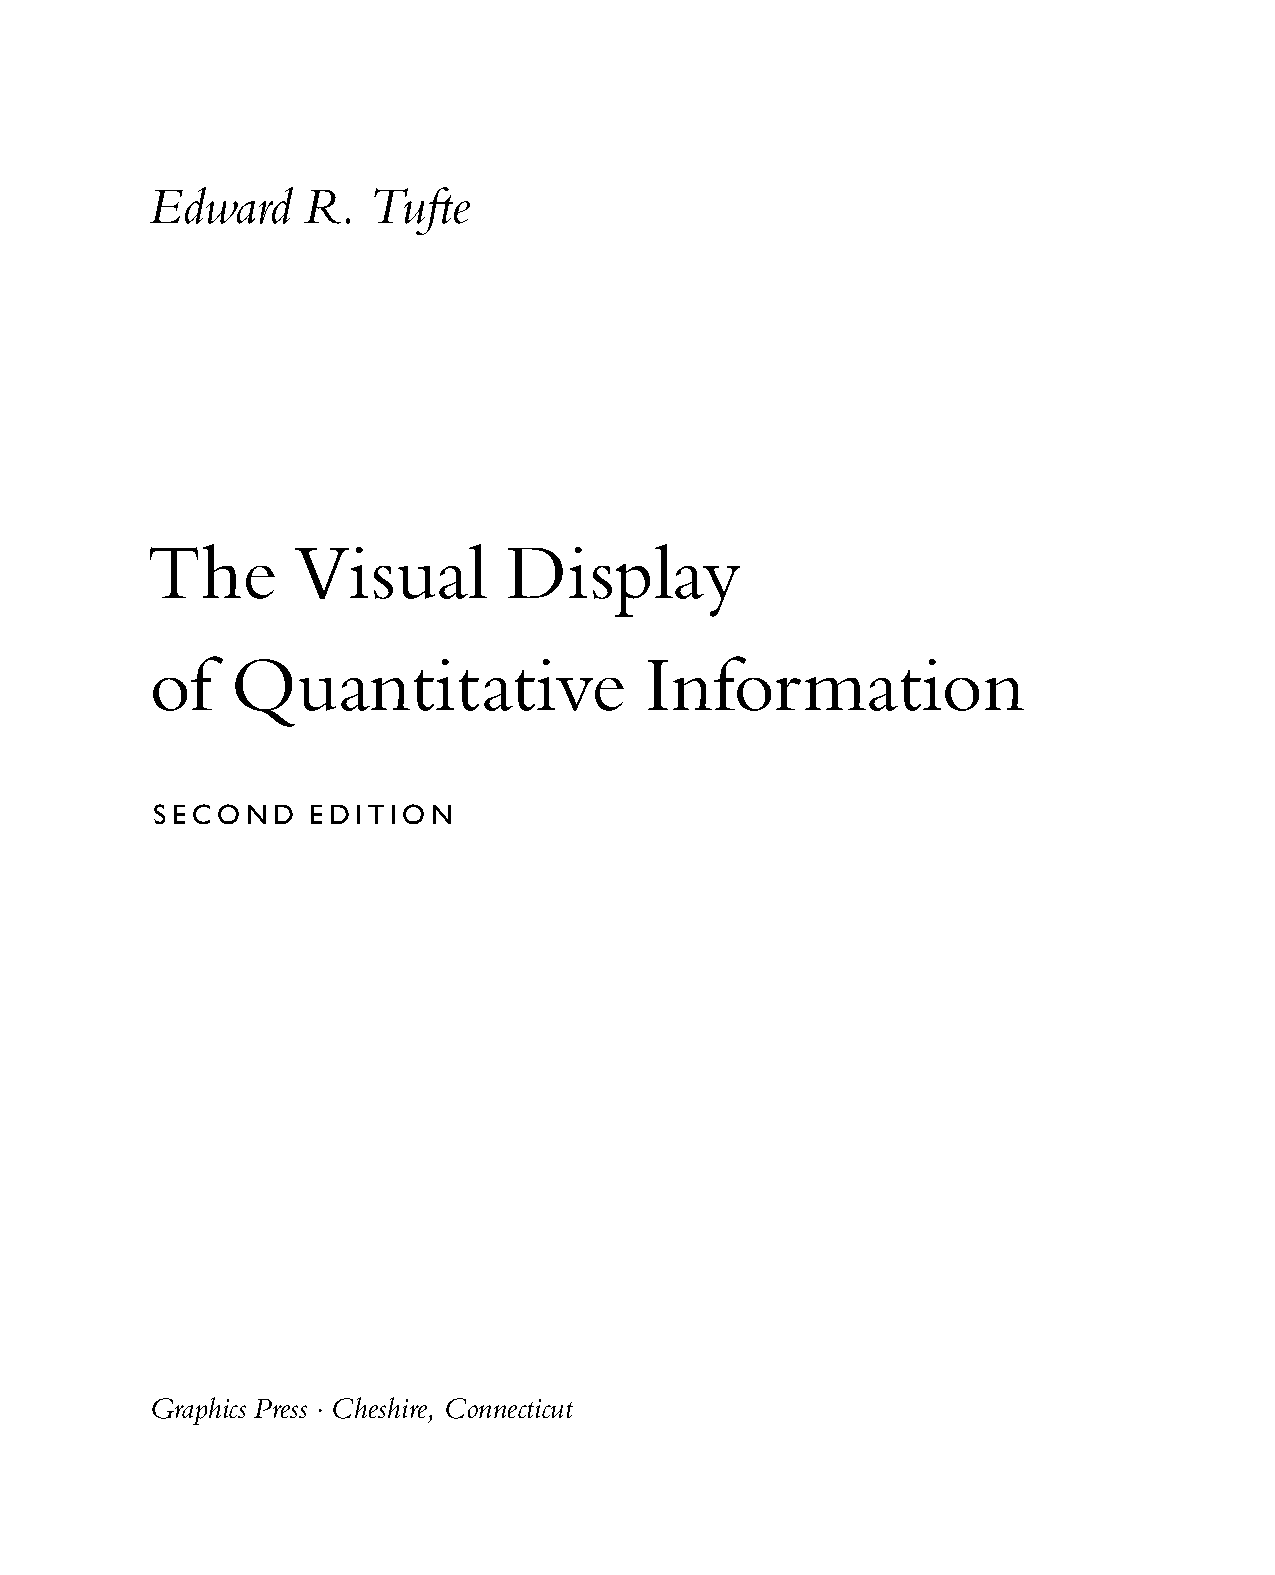
\includegraphics[width=0.45\linewidth]{vdqi-title.pdf}}
\hfill
\fbox{
\includegraphics[width=0.45\linewidth]{ei-title.pdf}}
\\\vspace{\baselineskip}
\fbox{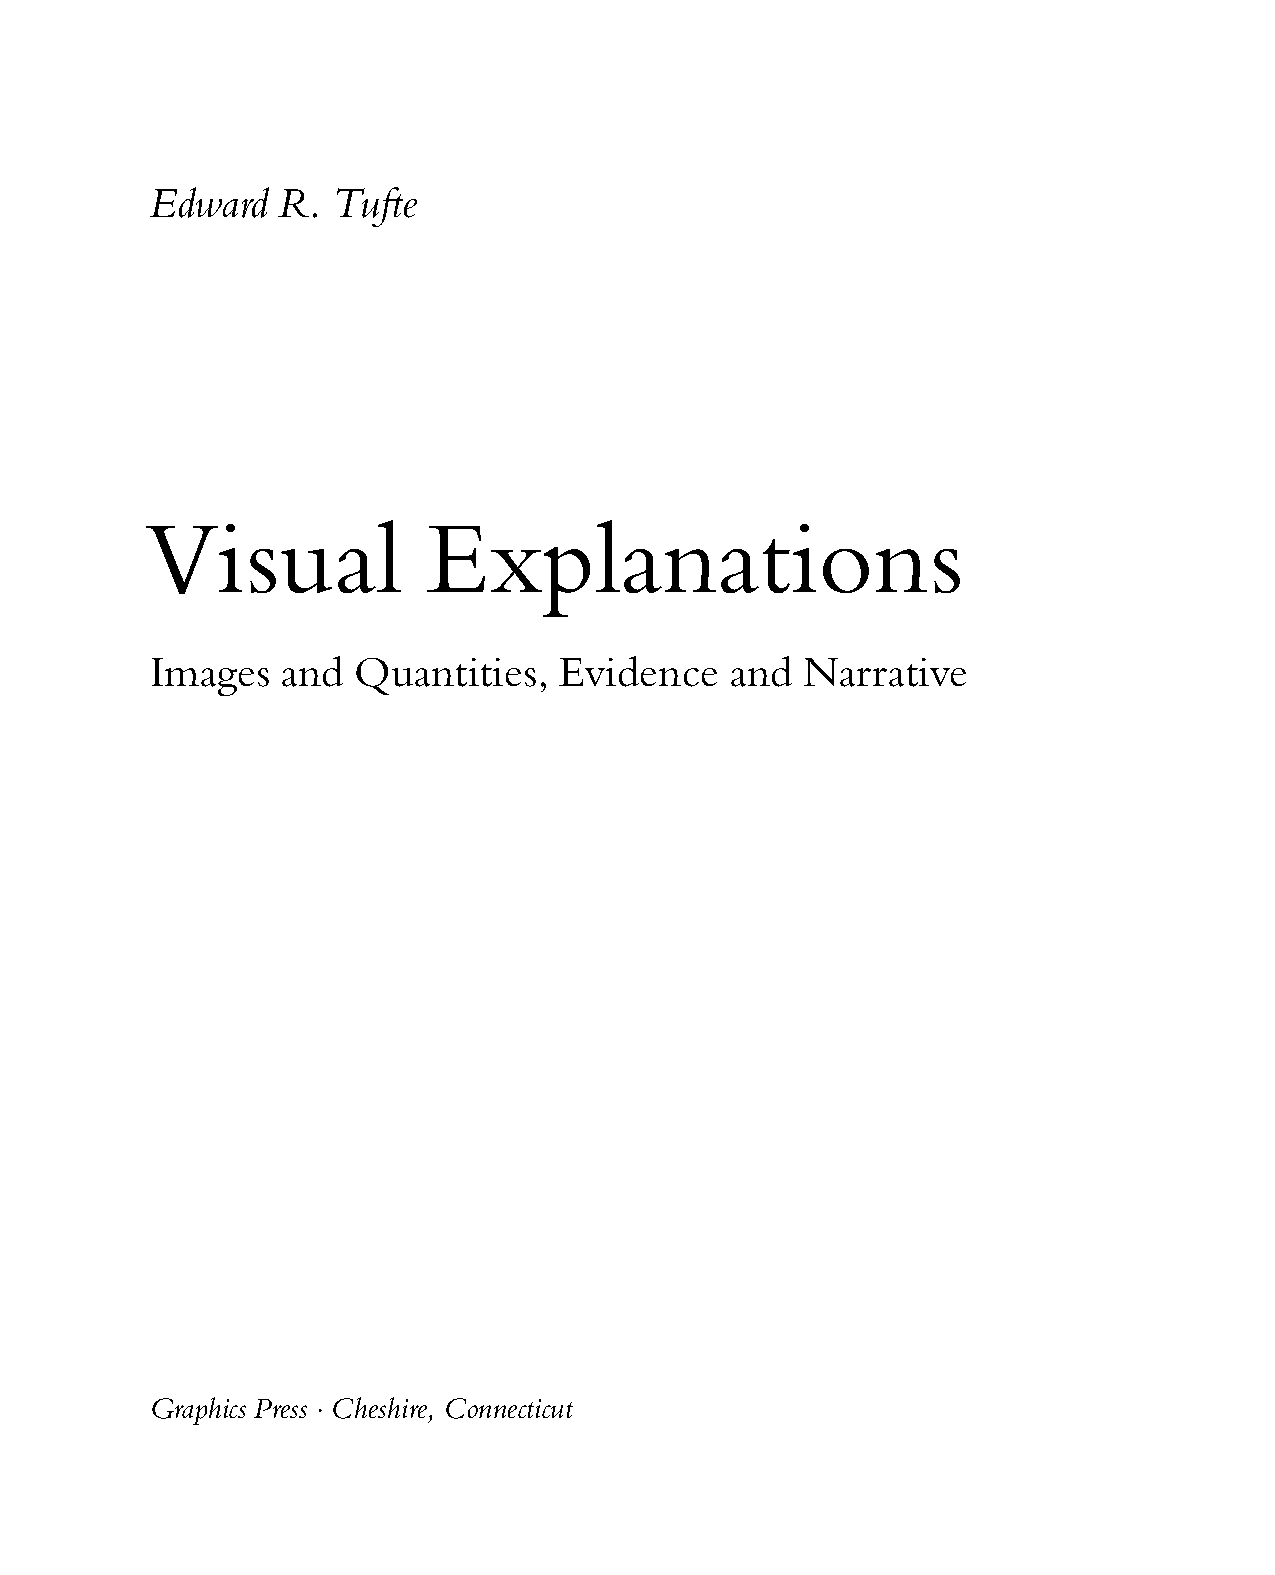
\includegraphics[width=0.45\linewidth]{ve-title.pdf}}
\hfill
\fbox{
\includegraphics[width=0.45\linewidth]{be-title.pdf}}
\end{figure*}

\newthought{The tables of contents} in Tufte's books give us our first
glimpse of the structure of the main matter.  \VDQI is split into two
parts, each containing some number of chapters.  His other three books only
contain chapters---they're not broken into parts.

\begin{figure*}[p]\index{table of contents}
\fbox{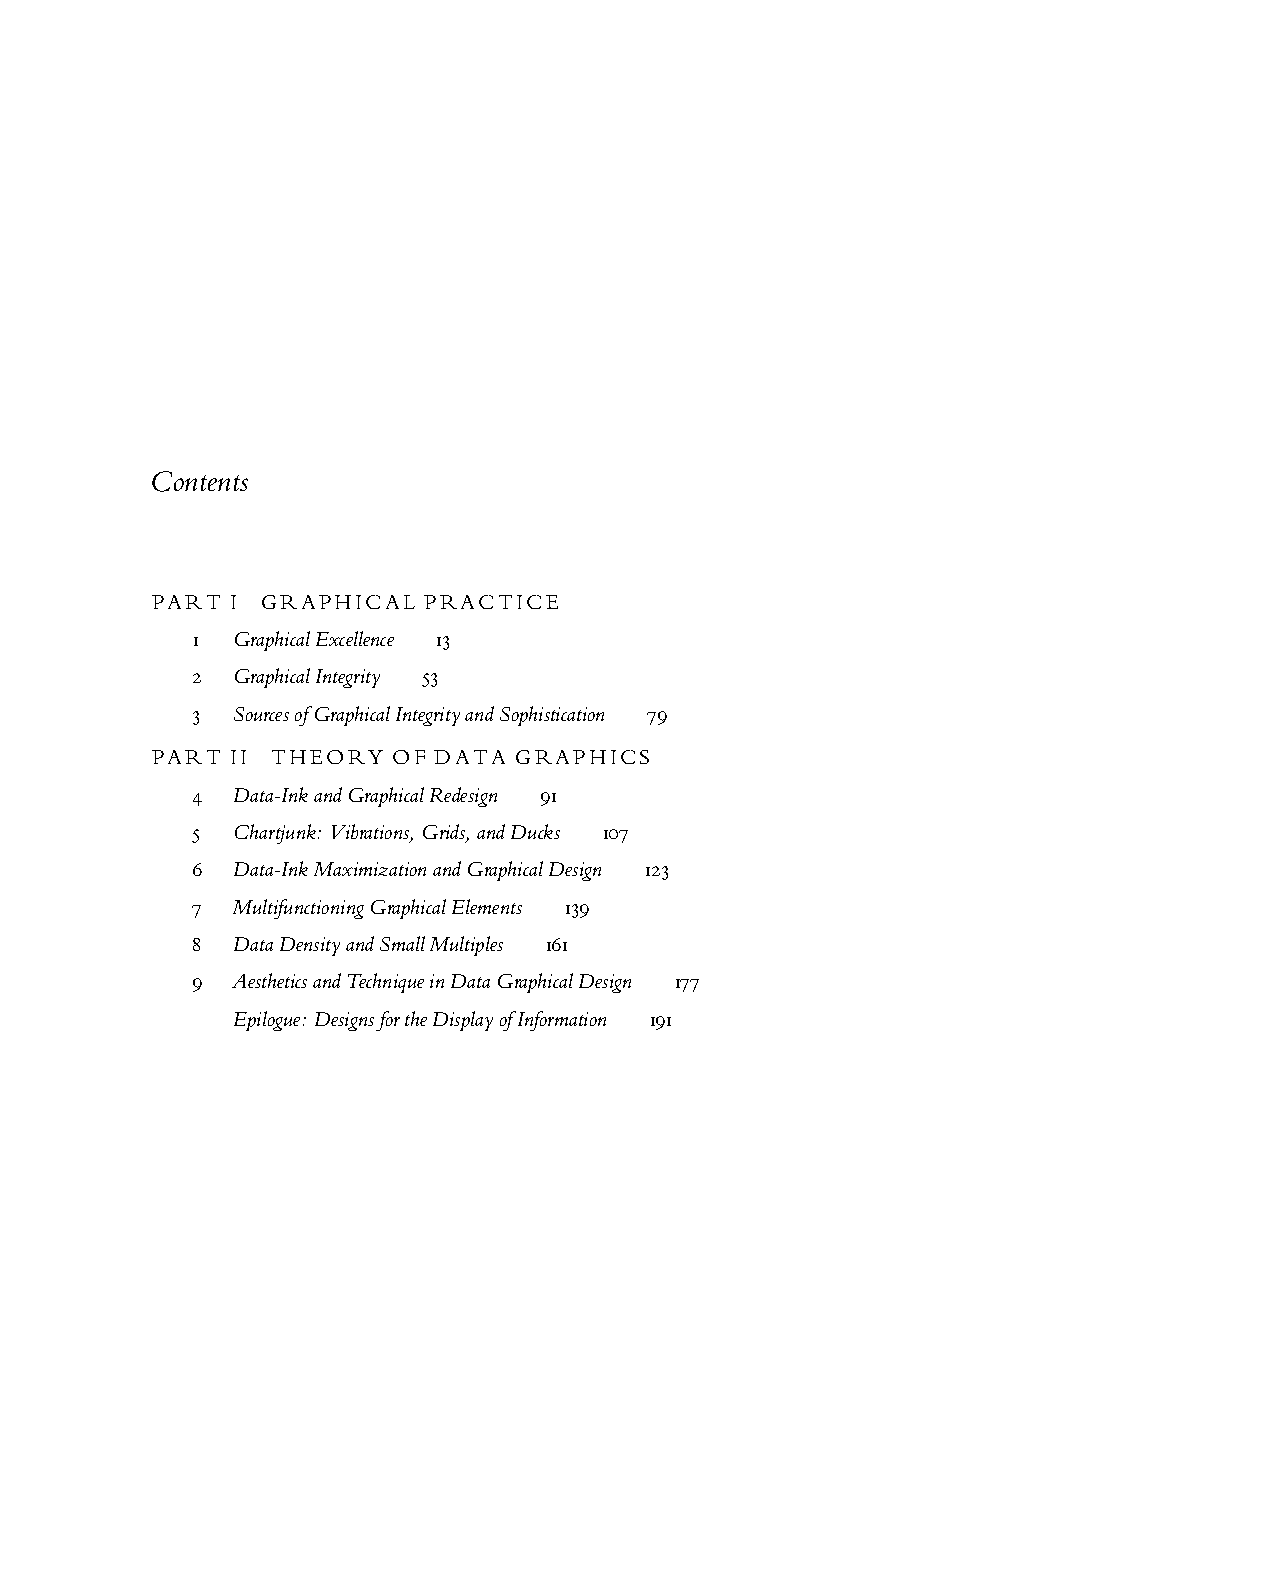
\includegraphics[width=0.45\linewidth]{vdqi-contents.pdf}}
\hfill
\fbox{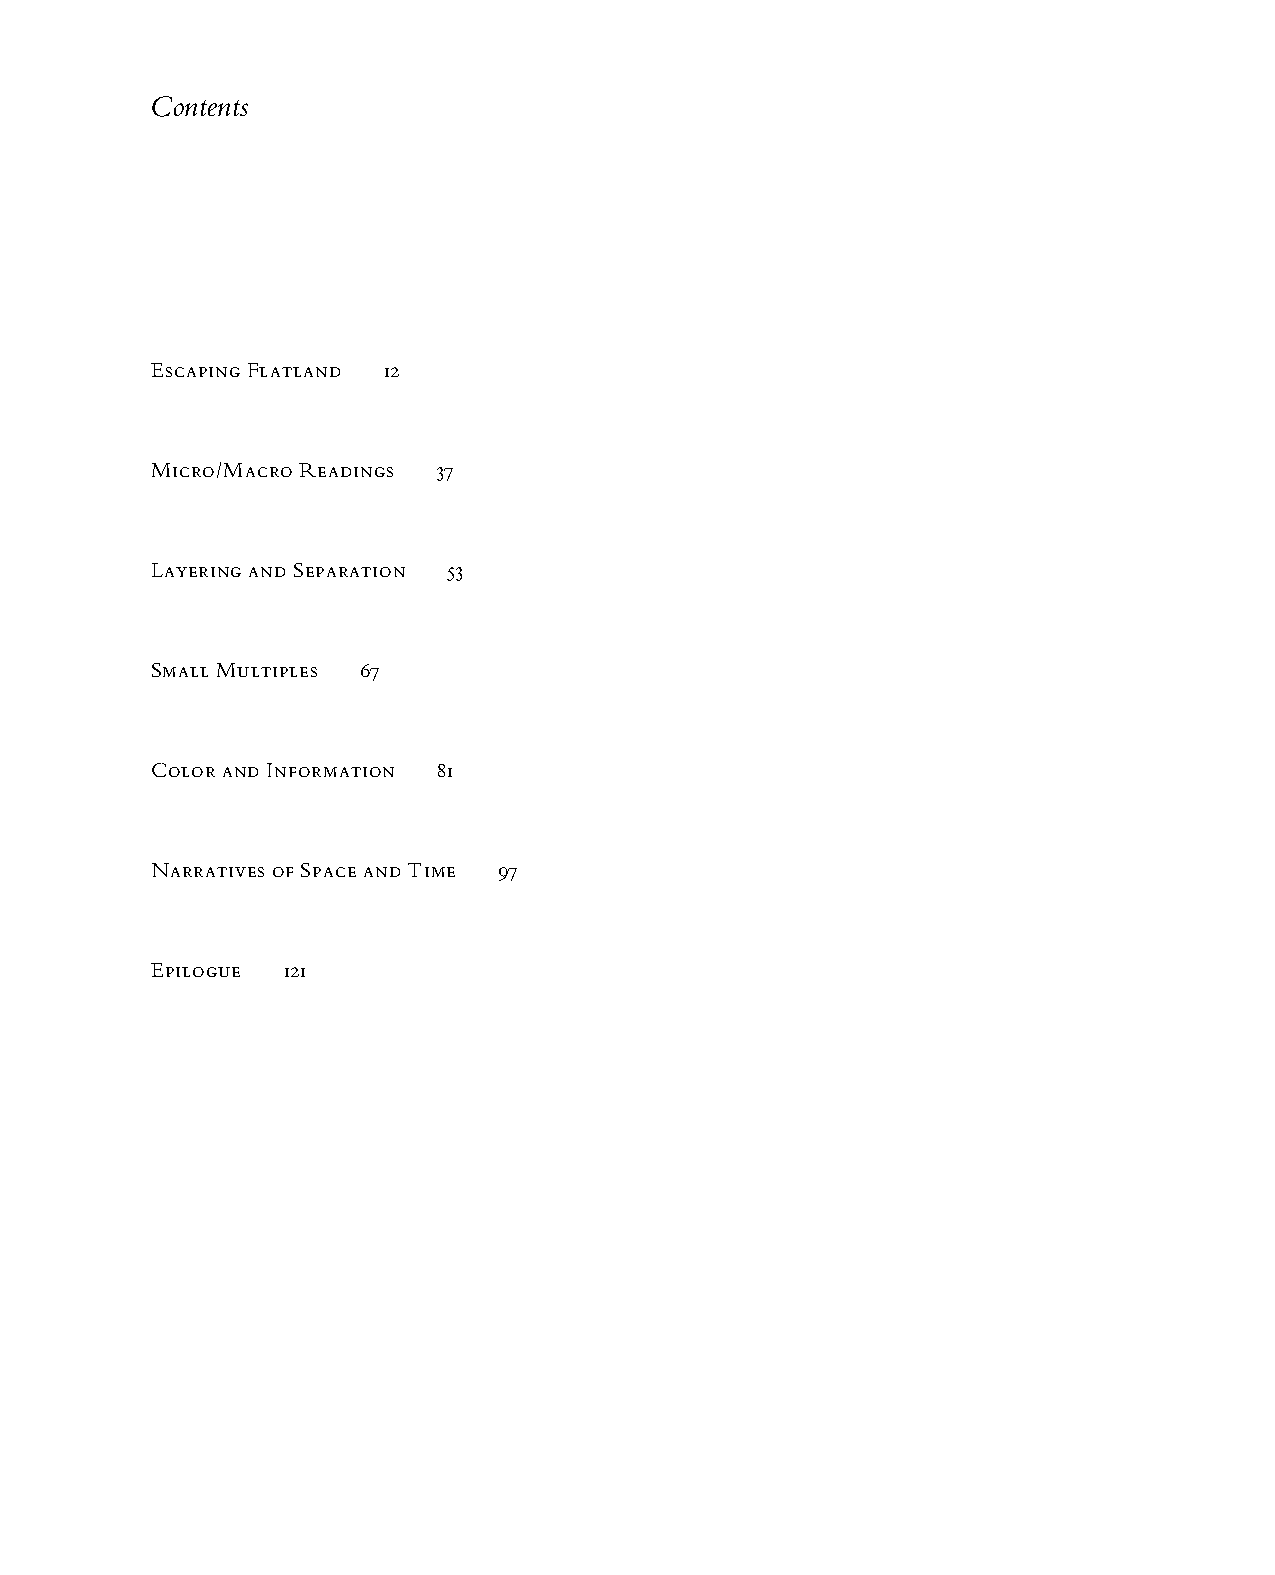
\includegraphics[width=0.45\linewidth]{ei-contents.pdf}}
\\\vspace{\baselineskip}
\fbox{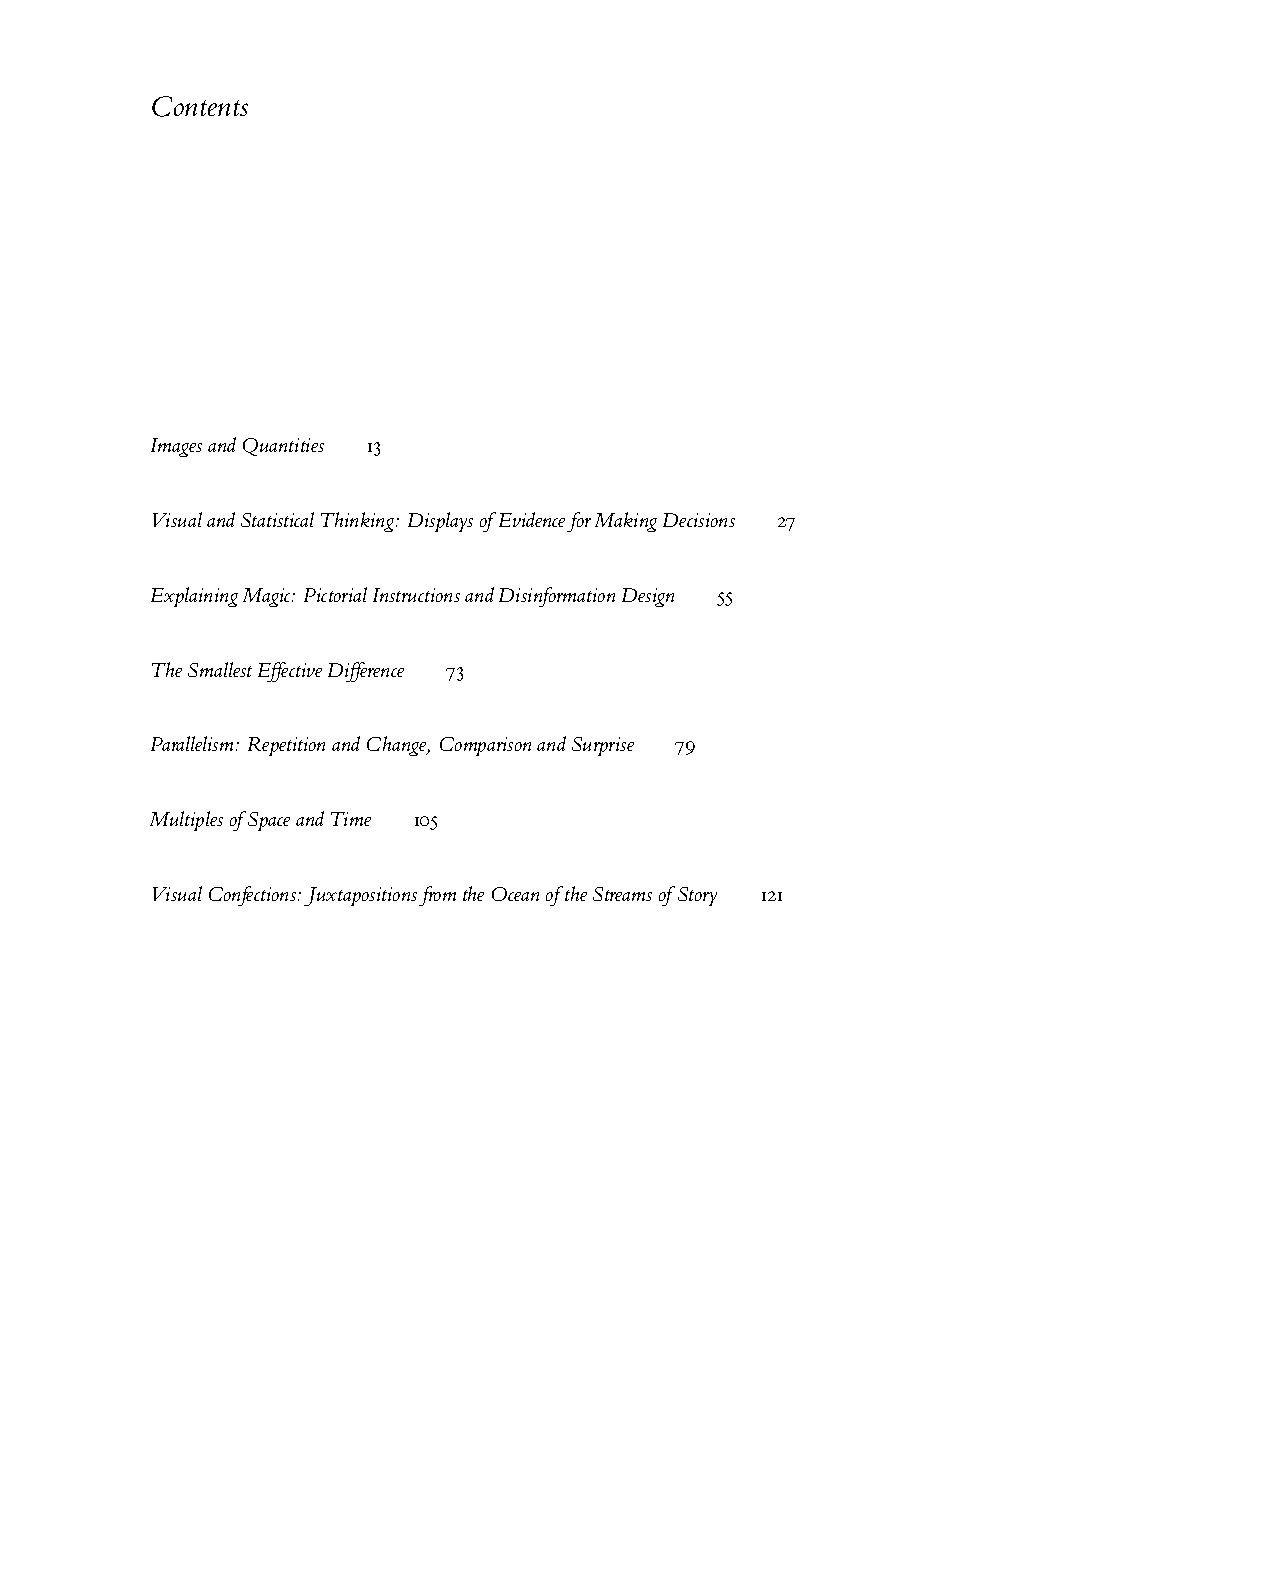
\includegraphics[width=0.45\linewidth]{ve-contents.pdf}}
\hfill
\fbox{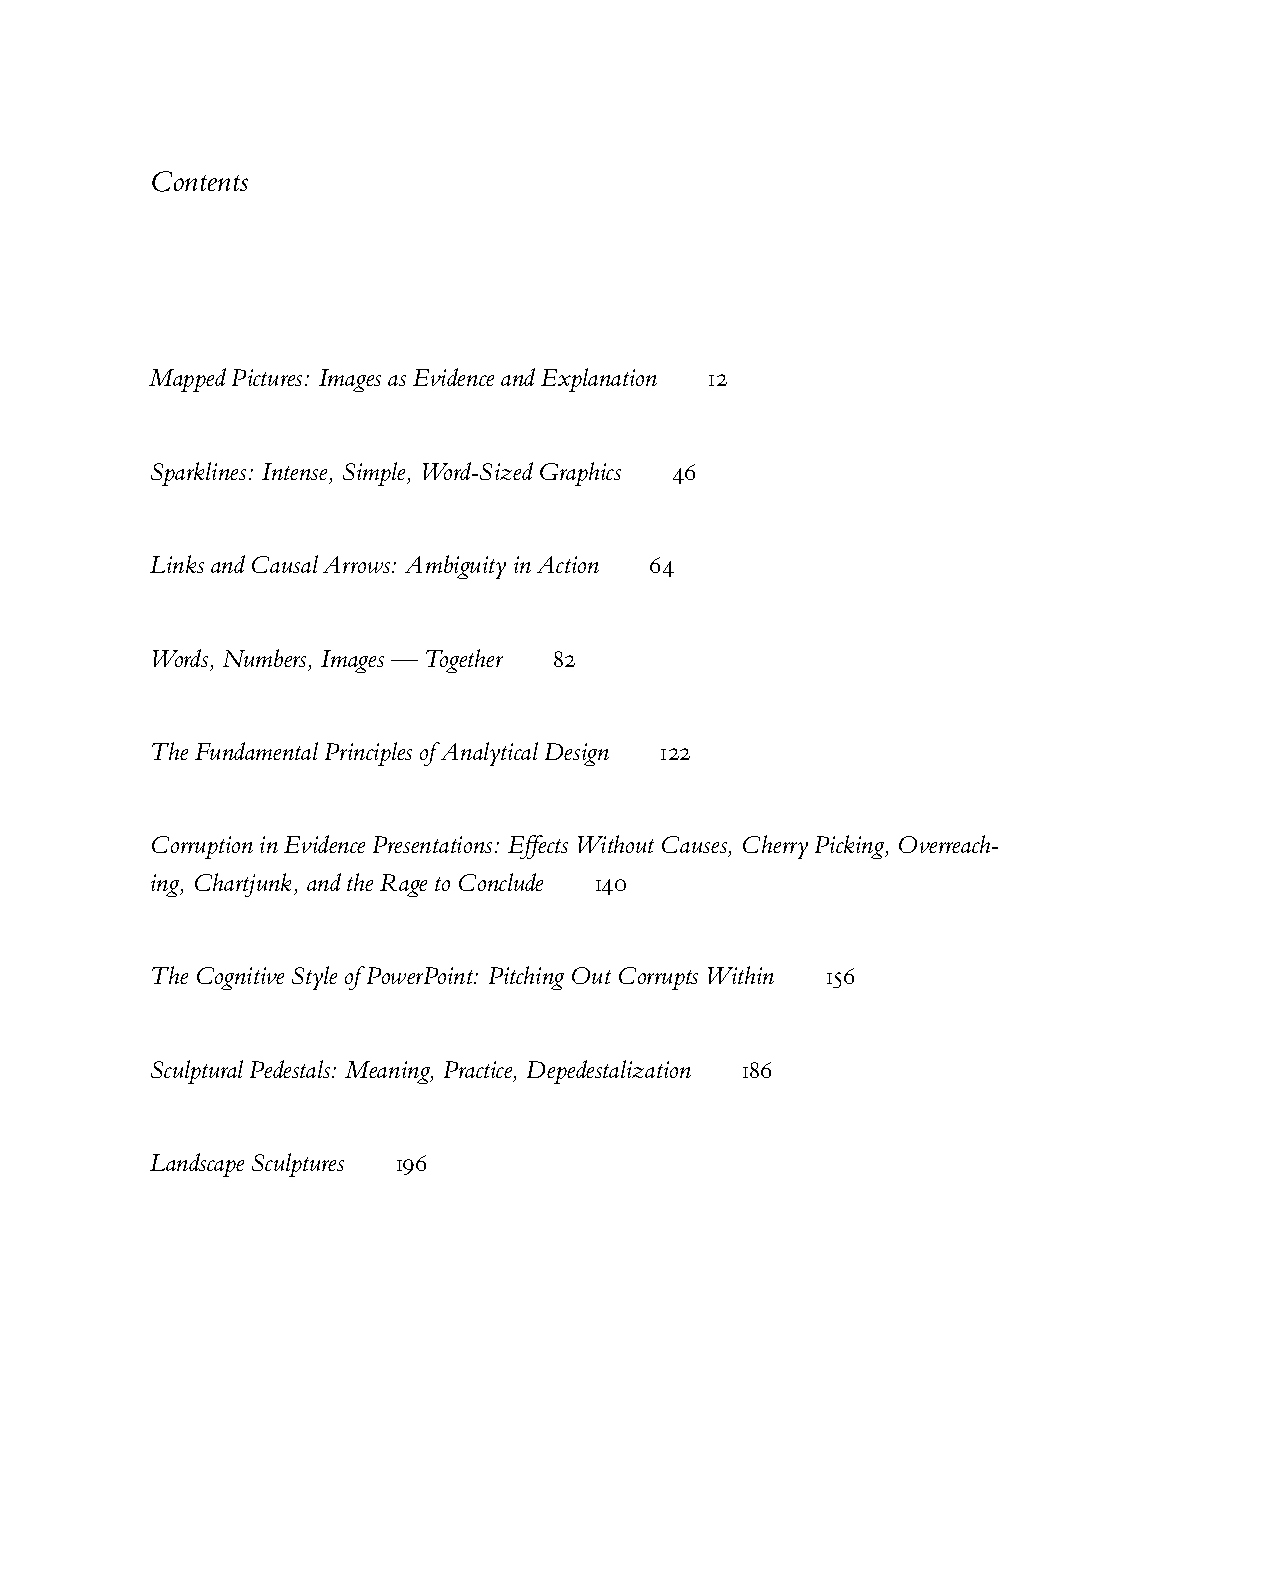
\includegraphics[width=0.45\linewidth]{be-contents.pdf}}
\end{figure*}


\section{Typefaces}\label{sec:typefaces1}\index{typefaces}
\index{fonts|see{typefaces}}

Tufte's books primarily use two typefaces: Bembo and Gill Sans.  Bembo is used
for the headings and body text, while Gill Sans is used for the title page and
opening epigraphs in \BE.

Since neither Bembo nor Gill Sans are available in default \LaTeX{}
installations, the \TL document classes default to using Palatino and
Helvetica, respectively.  In addition, the Bera Mono typeface is used for
\texttt{monospaced} type.

The following font sizes are defined by the \TL classes:

\begin{table}[h]\index{typefaces!sizes}
  \footnotesize%
  \begin{center}
    \begin{tabular}{lccl}
      \toprule
      \LaTeX{} size & Font size & Leading & Used for \\
      \midrule
      \verb+\tiny+         &  5 &  6 & sidenote numbers \\
      \verb+\scriptsize+   &  7 &  8 & \na \\
      \verb+\footnotesize+ &  8 & 10 & sidenotes, captions \\
      \verb+\small+        &  9 & 12 & quote, quotation, and verse environments \\
      \verb+\normalsize+   & 10 & 14 & body text \\
      \verb+\large+        & 11 & 15 & \textsc{b}-heads \\
      \verb+\Large+        & 12 & 16 & \textsc{a}-heads, \textsc{toc} entries, author, date \\
      \verb+\LARGE+        & 14 & 18 & handout title \\
      \verb+\huge+         & 20 & 30 & chapter heads \\
      \verb+\Huge+         & 24 & 36 & part titles \\
      \bottomrule
    \end{tabular}
  \end{center}
  \caption{A list of \LaTeX{} font sizes as defined by the \TL document classes.}
  \label{tab:font-sizes}
\end{table}

\section{Headings}\label{sec:headings1}\index{headings}

Tufte's books include the following heading levels: parts,
chapters,\sidenote{Parts and chapters are defined for the \texttt{tufte-book}
class only.}  sections, subsections, and paragraphs.  Not defined by default
are: sub-subsections and subparagraphs.

\begin{table}[h]
  \begin{center}
    \footnotesize%
    \begin{tabular}{lcr}
      \toprule
      Heading & Style & Size \\
      \midrule
      Part & roman & \measure{24}{36}{40} \\
      Chapter & italic & \measure{20}{30}{40} \\
      Section & italic & \measure{12}{16}{26} \\
      Subsection & italic & \measure{11}{15}{26} \\
      Paragraph & italic & 10/14 \\
      \bottomrule
    \end{tabular}
  \end{center}
  \caption{Heading styles used in \BE.}
  \label{tab:heading-styles}
\end{table}

\paragraph{Paragraph} Paragraph headings (as shown here) are introduced by
italicized text and separated from the main paragraph by a bit of space.

\section{Environments}

The following characteristics define the various environments:


\begin{table}[h]
  \begin{center}
    \footnotesize%
    \begin{tabular}{lcl}
      \toprule
      Environment & Font size & Notes \\
      \midrule
      Body text & \measure{10}{14}{26} & \\
      Block quote & \measure{9}{12}{24} & Block indent (left and right) by \unit[1]{pc} \\
      Sidenotes & \measure{8}{10}{12} & Sidenote number is set inline, followed by word space \\
      Captions & \measure{8}{10}{12} &  \\
      \bottomrule
    \end{tabular}
  \end{center}
  \caption{Environment styles used in \BE.}
  \label{tab:environment-styles}
\end{table}


\chapter[On the Use of the tufte-book Document Class]{On the Use of the \texttt{tufte-book} Document Class}
\label{ch:tufte-book}

The \TL document classes define a style similar to the
style Edward Tufte uses in his books and handouts.  Tufte's style is known
for its extensive use of sidenotes, tight integration of graphics with
text, and well-set typography.  This document aims to be at once a
demonstration of the features of the \TL document classes
and a style guide to their use.

\section{Page Layout}\label{sec:page-layout}
\subsection{Headings}\label{sec:headings}\index{headings}
This style provides \textsc{a}- and \textsc{b}-heads (that is,
\Verb|\section| and \Verb|\subsection|), demonstrated above.

If you need more than two levels of section headings, you'll have to define
them yourself at the moment; there are no pre-defined styles for anything below
a \Verb|\subsection|.  As Bringhurst points out in \textit{The Elements of
Typographic Style},\cite{Bringhurst2005} you should ``use as many levels of
headings as you need: no more, and no fewer.''

The \TL classes will emit an error if you try to use
\linebreak\Verb|\subsubsection| and smaller headings.

% let's start a new thought -- a new section
\newthought{In his later books},\cite{Tufte2006} Tufte
starts each section with a bit of vertical space, a non-indented paragraph,
and sets the first few words of the sentence in \textsc{small caps}.  To
accomplish this using this style, use the \doccmddef{newthought} command:
\begin{docspec}
  \doccmd{newthought}\{In his later books\}, Tufte starts\ldots
\end{docspec}


\section{Sidenotes}\label{sec:sidenotes}
One of the most prominent and distinctive features of this style is the
extensive use of sidenotes.  There is a wide margin to provide ample room
for sidenotes and small figures.  Any \doccmd{footnote}s will automatically
be converted to sidenotes.\footnote{This is a sidenote that was entered
using the \texttt{\textbackslash footnote} command.}  If you'd like to place ancillary
information in the margin without the sidenote mark (the superscript
number), you can use the \doccmd{marginnote} command.\marginnote{This is a
margin note.  Notice that there isn't a number preceding the note, and
there is no number in the main text where this note was written.}

The specification of the \doccmddef{sidenote} command is:
\begin{docspec}
  \doccmd{sidenote}[\docopt{number}][\docopt{offset}]\{\docarg{Sidenote text.}\}
\end{docspec}

Both the \docopt{number} and \docopt{offset} arguments are optional.  If you
provide a \docopt{number} argument, then that number will be used as the
sidenote number.  It will change of the number of the current sidenote only and
will not affect the numbering sequence of subsequent sidenotes.

Sometimes a sidenote may run over the top of other text or graphics in the
margin space.  If this happens, you can adjust the vertical position of the
sidenote by providing a dimension in the \docopt{offset} argument.  Some
examples of valid dimensions are:
\begin{docspec}
  \ttfamily 1.0in \qquad 2.54cm \qquad 254mm \qquad 6\Verb|\baselineskip|
\end{docspec}
If the dimension is positive it will push the sidenote down the page; if the
dimension is negative, it will move the sidenote up the page.

While both the \docopt{number} and \docopt{offset} arguments are optional, they
must be provided in order.  To adjust the vertical position of the sidenote
while leaving the sidenote number alone, use the following syntax:
\begin{docspec}
  \doccmd{sidenote}[][\docopt{offset}]\{\docarg{Sidenote text.}\}
\end{docspec}
The empty brackets tell the \Verb|\sidenote| command to use the default
sidenote number.

If you \emph{only} want to change the sidenote number, however, you may
completely omit the \docopt{offset} argument:
\begin{docspec}
  \doccmd{sidenote}[\docopt{number}]\{\docarg{Sidenote text.}\}
\end{docspec}

The \doccmddef{marginnote} command has a similar \docarg{offset} argument:
\begin{docspec}
  \doccmd{marginnote}[\docopt{offset}]\{\docarg{Margin note text.}\}
\end{docspec}

\section{References}
References are placed alongside their citations as sidenotes,
as well.  This can be accomplished using the normal \doccmddef{cite}
command.\sidenote{The first paragraph of this document includes a citation.}

The complete list of references may also be printed automatically by using
the \doccmddef{bibliography} command.  (See the end of this document for an
example.)  If you do not want to print a bibliographyn at the end of your
document, use the \doccmddef{nobibliography} command in its place.  

To enter multiple citations at one location,\cite[-3\baselineskip]{Tufte2006,Tufte1990} you can
provide a list of keys separated by commas and the same optional vertical
offset argument: \Verb|\cite{Tufte2006,Tufte1990}|.  
\begin{docspec}
  \doccmd{cite}[\docopt{offset}]\{\docarg{bibkey1,bibkey2,\ldots}\}
\end{docspec}

\section{Figures and Tables}\label{sec:figures-and-tables}
Images and graphics play an integral role in Tufte's work.
In addition to the standard \docenvdef{figure} and \docenvdef{tabular} environments,
this style provides special figure and table environments for full-width
floats.

Full page--width figures and tables may be placed in \docenvdef{figure*} or
\docenvdef{table*} environments.  To place figures or tables in the margin,
use the \docenvdef{marginfigure} or \docenvdef{margintable} environments as follows
(see figure~\ref{fig:marginfig}):

\begin{marginfigure}%
  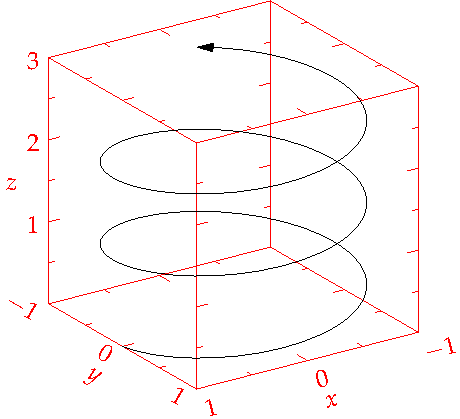
\includegraphics[width=\linewidth]{helix}
  \caption{This is a margin figure.  The helix is defined by 
    $x = \cos(2\pi z)$, $y = \sin(2\pi z)$, and $z = [0, 2.7]$.  The figure was
    drawn using Asymptote (\protect\url{http://asymptote.sf.net/}).}
  \label{fig:marginfig}
\end{marginfigure}

\begin{docspec}
\textbackslash begin\{marginfigure\}\\
  \qquad\textbackslash includegraphics\{helix\}\\
  \qquad\textbackslash caption\{This is a margin figure.\}\\
  \qquad\textbackslash label\{fig:marginfig\}\\
\textbackslash end\{marginfigure\}\\
\end{docspec}

The \docenv{marginfigure} and \docenv{margintable} environments accept an optional parameter \docopt{offset} that adjusts the vertical position of the figure or table.  See the ``\nameref{sec:sidenotes}'' section above for examples.  The specifications are:
\begin{docspec}
  \textbackslash{begin\{marginfigure\}[\docopt{offset}]}\\
  \qquad\ldots\\
  \textbackslash{end\{marginfigure\}}\\
  \mbox{}\\
  \textbackslash{begin\{margintable\}[\docopt{offset}]}\\
  \qquad\ldots\\
  \textbackslash{end\{margintable\}}\\
\end{docspec}

Figure~\ref{fig:fullfig} is an example of the \docenv{figure*}
environment and figure~\ref{fig:textfig} is an example of the normal
\docenv{figure} environment.

\begin{figure*}[h]
  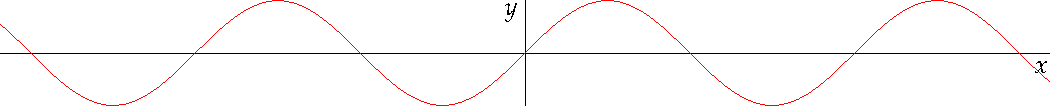
\includegraphics[width=\linewidth]{sine.pdf}%
  \caption{This graph shows $y = \sin x$ from about $x = [-10, 10]$.
  \emph{Notice that this figure takes up the full page width.}}%
  \label{fig:fullfig}%
\end{figure*}

\begin{figure}
  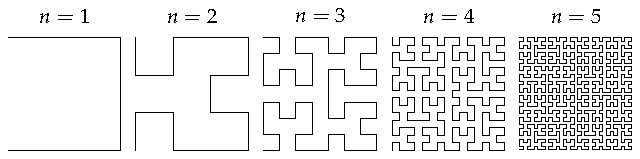
\includegraphics{hilbertcurves.pdf}
%  \checkparity This is an \pageparity\ page.%
  \caption[Hilbert curves of various degrees $n$.][6pt]{Hilbert curves of various degrees $n$. \emph{Notice that this figure only takes up the main textblock width.}}
  \label{fig:textfig}
  %\zsavepos{pos:textfig}
\end{figure}

As with sidenotes and marginnotes, a caption may sometimes require vertical
adjustment. The \doccmddef{caption} command now takes a second optional
argument that enables you to do this by providing a dimension \docopt{offset}.
You may specify the caption in any one of the following forms:
\begin{docspec}
  \doccmd{caption}\{\docarg{long caption}\}\\
  \doccmd{caption}[\docarg{short caption}]\{\docarg{long caption}\}\\
  \doccmd{caption}[][\docopt{offset}]\{\docarg{long caption}\}\\
  \doccmd{caption}[\docarg{short caption}][\docopt{offset}]%
                  \{\docarg{long caption}\}
\end{docspec}
A positive \docopt{offset} will push the caption down the page. The short
caption, if provided, is what appears in the list of figures/tables, otherwise
the ``long'' caption appears there. Note that although the arguments
\docopt{short caption} and \docopt{offset} are both optional, they must be
provided in order. Thus, to specify an \docopt{offset} without specifying a
\docopt{short caption}, you must include the first set of empty brackets
\Verb|[]|, which tell \doccmd{caption} to use the default ``long'' caption. As
an example, the caption to figure~\ref{fig:textfig} above was given in the form
\begin{docspec}
  \doccmd{caption}[Hilbert curves...][6pt]\{Hilbert curves...\}
\end{docspec}

Table~\ref{tab:normaltab} shows table created with the \docpkg{booktabs}
package.  Notice the lack of vertical rules---they serve only to clutter
the table's data.

\begin{table}[ht]
  \centering
  \fontfamily{ppl}\selectfont
  \begin{tabular}{ll}
    \toprule
    Margin & Length \\
    \midrule
    Paper width & \unit[8\nicefrac{1}{2}]{inches} \\
    Paper height & \unit[11]{inches} \\
    Textblock width & \unit[6\nicefrac{1}{2}]{inches} \\
    Textblock/sidenote gutter & \unit[\nicefrac{3}{8}]{inches} \\
    Sidenote width & \unit[2]{inches} \\
    \bottomrule
  \end{tabular}
  \caption{Here are the dimensions of the various margins used in the Tufte-handout class.}
  \label{tab:normaltab}
  %\zsavepos{pos:normaltab}
\end{table}

\newthought{Occasionally} \LaTeX{} will generate an error message:\label{err:too-many-floats}
\begin{docspec}
  Error: Too many unprocessed floats
\end{docspec}
\LaTeX{} tries to place floats in the best position on the page.  Until it's
finished composing the page, however, it won't know where those positions are.
If you have a lot of floats on a page (including sidenotes, margin notes,
figures, tables, etc.), \LaTeX{} may run out of ``slots'' to keep track of them
and will generate the above error.

\LaTeX{} initially allocates 18 slots for storing floats.  To work around this
limitation, the \TL document classes provide a \doccmddef{morefloats} command
that will reserve more slots.

The first time \doccmd{morefloats} is called, it allocates an additional 34
slots.  The second time \doccmd{morefloats} is called, it allocates another 26
slots.

The \doccmd{morefloats} command may only be used two times.  Calling it a
third time will generate an error message.  (This is because we can't safely
allocate many more floats or \LaTeX{} will run out of memory.)

If, after using the \doccmd{morefloats} command twice, you continue to get the
\texttt{Too many unprocessed floats} error, there are a couple things you can
do.

The \doccmddef{FloatBarrier} command will immediately process all the floats
before typesetting more material.  Since \doccmd{FloatBarrier} will start a new
paragraph, you should place this command at the beginning or end of a
paragraph.

The \doccmddef{clearpage} command will also process the floats before
continuing, but instead of starting a new paragraph, it will start a new page.

You can also try moving your floats around a bit: move a figure or table to the
next page or reduce the number of sidenotes.  (Each sidenote actually uses
\emph{two} slots.)

After the floats have placed, \LaTeX{} will mark those slots as unused so they
are available for the next page to be composed.

\section{Captions}
You may notice that the captions are sometimes misaligned.
Due to the way \LaTeX's float mechanism works, we can't know for sure where it
decided to put a float. Therefore, the \TL document classes provide commands to
override the caption position.

\paragraph{Vertical alignment} To override the vertical alignment, use the
\doccmd{setfloatalignment} command inside the float environment.  For
example:

\begin{fullwidth}
\begin{docspec}
  \textbackslash begin\{figure\}[btp]\\
  \qquad \textbackslash includegraphics\{sinewave\}\\
  \qquad \textbackslash caption\{This is an example of a sine wave.\}\\
  \qquad \textbackslash label\{fig:sinewave\}\\
  \qquad \hlred{\textbackslash setfloatalignment\{b\}\% forces caption to be bottom-aligned}\\
  \textbackslash end\{figure\}
\end{docspec}
\end{fullwidth}

\noindent The syntax of the \doccmddef{setfloatalignment} command is:

\begin{docspec}
  \doccmd{setfloatalignment}\{\docopt{pos}\}
\end{docspec}

\noindent where \docopt{pos} can be either \texttt{b} for bottom-aligned
captions, or \texttt{t} for top-aligned captions.

\paragraph{Horizontal alignment}\label{par:overriding-horizontal}
To override the horizontal alignment, use either the \doccmd{forceversofloat}
or the \doccmd{forcerectofloat} command inside of the float environment.  For
example:

\begin{fullwidth}
\begin{docspec}
  \textbackslash begin\{figure\}[btp]\\
  \qquad \textbackslash includegraphics\{sinewave\}\\
  \qquad \textbackslash caption\{This is an example of a sine wave.\}\\
  \qquad \textbackslash label\{fig:sinewave\}\\
  \qquad \hlred{\textbackslash forceversofloat\% forces caption to be set to the left of the float}\\
  \textbackslash end\{figure\}
\end{docspec}
\end{fullwidth}

The \doccmddef{forceversofloat} command causes the algorithm to assume the
float has been placed on a verso page---that is, a page on the left side of a
two-page spread.  Conversely, the \doccmddef{forcerectofloat} command causes
the algorithm to assume the float has been placed on a recto page---that is, a
page on the right side of a two-page spread.


\section{Full-width text blocks}

In addition to the new float types, there is a \docenvdef{fullwidth}
environment that stretches across the main text block and the sidenotes
area.

\begin{Verbatim}
\begin{fullwidth}
Lorem ipsum dolor sit amet...
\end{fullwidth}
\end{Verbatim}

\begin{fullwidth}
\small\itshape\lipsum[1]
\end{fullwidth}

\section{Typography}\label{sec:typography}

\subsection{Typefaces}\label{sec:typefaces}\index{typefaces}
If the Palatino, \textsf{Helvetica}, and \texttt{Bera Mono} typefaces are installed, this style
will use them automatically.  Otherwise, we'll fall back on the Computer Modern
typefaces.

\subsection{Letterspacing}\label{sec:letterspacing}
This document class includes two new commands and some improvements on
existing commands for letterspacing.

When setting strings of \allcaps{ALL CAPS} or \smallcaps{small caps}, the
letter\-spacing---that is, the spacing between the letters---should be
increased slightly.\cite[][p.32]{Bringhurst2005} The \doccmddef{allcaps} command has proper letterspacing for
strings of \allcaps{FULL CAPITAL LETTERS}, and the \doccmddef{smallcaps} command
has letterspacing for \smallcaps{small capital letters}.  These commands
will also automatically convert the case of the text to upper- or
lowercase, respectively.

The \doccmddef{textsc} command has also been redefined to include
letterspacing.  The case of the \doccmd{textsc} argument is left as is,
however.  This allows one to use both uppercase and lowercase letters:
\textsc{The Initial Letters Of The Words In This Sentence Are Capitalized.}



\section{Document Class Options}\label{sec:options}

\index{class options|(}
The \doccls{tufte-book} class is based on the \LaTeX\ \doccls{book}
document class.  Therefore, you can pass any of the typical book
options.  There are a few options that are specific to the
\doccls{tufte-book} document class, however.

The \docclsoptdef{a4paper} option will set the paper size to \smallcaps{A4} instead of
the default \smallcaps{US} letter size.

The \docclsoptdef{sfsidenotes} option will set the sidenotes and title block in a 
\textsf{sans serif} typeface instead of the default roman.

The \docclsoptdef{twoside} option will modify the running heads so that the page
number is printed on the outside edge (as opposed to always printing the page
number on the right-side edge in \docclsoptdef{oneside} mode).  

The \docclsoptdef{symmetric} option typesets the sidenotes on the outside edge of
the page.  This is how books are traditionally printed, but is contrary to
Tufte's book design which sets the sidenotes on the right side of the page.
This option implicitly sets the \docclsopt{twoside} option.

The \docclsoptdef{justified} option sets all the text fully justified (flush left
and right).  The default is to set the text ragged right.  
The body text of Tufte's books are set ragged right.  This prevents
needless hyphenation and makes it easier to read the text in the slightly
narrower column.

The \docclsoptdef{bidi} option loads the \docpkg{bidi} package which is used with
\tXeLaTeX\ to typeset bi-directional text.  Since the \docpkg{bidi}
package needs to be loaded before the sidenotes and cite commands are defined,
it can't be loaded in the document preamble.

The \docclsoptdef{debug} option causes the \TL classes to output debug
information to the log file which is useful in troubleshooting bugs.  It will
also cause the graphics to be replaced by outlines.

The \docclsoptdef{nofonts} option prevents the \TL classes from
automatically loading the Palatino and Helvetica typefaces.  You should use
this option if you wish to load your own fonts.  If you're using \tXeLaTeX, this
option is implied (\ie, the Palatino and Helvetica fonts aren't loaded if you
use \tXeLaTeX).  

The \docclsoptdef{nols} option inhibits the letterspacing code.  The \TL\
classes try to load the appropriate letterspacing package (either pdf\TeX's
\docpkg{letterspace} package or the \docpkg{soul} package).  If you're using
\tXeLaTeX\ with \docpkg{fontenc}, however, you should configure your own
letterspacing.  

The \docclsoptdef{notitlepage} option causes \doccmd{maketitle} to generate a title
block instead of a title page.  The \doccls{book} class defaults to a title
page and the \doccls{handout} class defaults to the title block.  There is an
analogous \docclsoptdef{titlepage} option that forces \doccmd{maketitle} to
generate a full title page instead of the title block.

The \docclsoptdef{notoc} option suppresses \TL's custom table of contents
(\textsc{toc}) design.  The current \textsc{toc} design only shows unnumbered
chapter titles; it doesn't show sections or subsections.  The \docclsopt{notoc}
option will revert to \LaTeX's \textsc{toc} design.

The \docclsoptdef{nohyper} option prevents the \docpkg{hyperref} package from
being loaded.  The default is to load the \docpkg{hyperref} package and use the
\doccmd{title} and \doccmd{author} contents as metadata for the generated
\textsc{pdf}.

\index{class options|)}



\chapter[Customizing Tufte-LaTeX]{Customizing \TL}
\label{ch:customizing}

The \TL document classes are designed to closely emulate Tufte's book
design by default.  However, each document is different and you may encounter
situations where the default settings are insufficient.  This chapter explores
many of the ways you can adjust the \TL document classes to better fit
your needs.

\section{File Hooks}
\label{sec:filehooks}

\index{file hooks|(}
If you create many documents using the \TL classes, it's easier to
store your customizations in a separate file instead of copying them into the
preamble of each document.  The \TL classes provide three file hooks:
\docfilehook{tufte-common-local.tex}{common}, \docfilehook{tufte-book-local.tex}{book}, and
\docfilehook{tufte-handout-local.tex}{handout}.\sloppy

\begin{description}
  \item[\docfilehook{tufte-common-local.tex}{common}]
    If this file exists, it will be loaded by all of the \TL document
    classes just prior to any document-class-specific code.  If your
    customizations or code should be included in both the book and handout
    classes, use this file hook.
  \item[\docfilehook{tufte-book-local.tex}{book}] 
    If this file exists, it will be loaded after all of the common and
    book-specific code has been read.  If your customizations apply only to the
    book class, use this file hook.
  \item[\docfilehook{tufte-common-handout.tex}{handout}] 
    If this file exists, it will be loaded after all of the common and
    handout-specific code has been read.  If your customizations apply only to
    the handout class, use this file hook.
\end{description}

\index{file hooks|)}

\section{Numbered Section Headings}
\label{sec:numbered-sections}
\index{headings!numbered}

While Tufte dispenses with numbered headings in his books, if you require them,
they can be anabled by changing the value of the \doccounter{secnumdepth}
counter.  From the table below, select the heading level at which numbering
should stop and set the \doccounter{secnumdepth} counter to that value.  For
example, if you want parts and chapters numbered, but don't want numbering for
sections or subsections, use the command:
\begin{docspec}
  \doccmd{setcounter}\{secnumdepth\}\{0\}
\end{docspec}

The default \doccounter{secnumdepth} for the \TL document classes is $-1$.

\begin{table}
  \footnotesize
  \begin{center}
    \begin{tabular}{lr}
      \toprule
      Heading level & Value \\
      \midrule
      Part (in \doccls{tufte-book}) & $-1$ \\
      Part (in \doccls{tufte-handout}) & $0$ \\
      Chapter (only in \doccls{tufte-book}) & $0$ \\
      Section & $1$ \\
      Subsection & $2$ \\
      Subsubsection & $3$ \\
      Paragraph & $4$ \\
      Subparagraph & $5$ \\
      \bottomrule
    \end{tabular}
  \end{center}
  \caption{Heading levels used with the \texttt{secnumdepth} counter.}
\end{table}

\section{Changing the Paper Size}
\label{sec:paper-size}

The \TL classes currently only provide three paper sizes: \textsc{a4},
\textsc{b5}, and \textsc{us} letter.  To specify a different paper size (and/or
margins), use the \doccmd[geometry]{geometrysetup} command in the preamble of your
document (or one of the file hooks).  The full documentation of the
\doccmd{geometrysetup} command may be found in the \docpkg{geometry} package
documentation.\cite[-1em][p.33]{pkg-geometry}


\section{Customizing Marginal Material}
\label{sec:marginal-material}

Marginal material includes sidenotes, citations, margin notes, and captions.
Normally, the justification of the marginal material follows the justification
of the body text.  If you specify the \docclsopt{justified} document class
option, all of the margin material will be fully justified as well.  If you
don't specify the \docclsopt{justified} option, then the marginal material will
be set ragged right.

You can set the justification of the marginal material separately from the body
text using the following document class options: \docclsopt{sidenote},
\docclsopt{marginnote}, \docclsopt{caption}, \docclsopt{citation}, and
\docclsopt{marginals}.  Each option refers to its obviously corresponding
marginal material type.  The \docclsopt{marginals} option simultaneously sets
the justification on all four marginal material types.

Each of the document class options takes one of five justification types:
\begin{description}
  \item[\docclsopt{justified}] Fully justifies the text (sets it flush left and
    right).
  \item[\docclsopt{raggedleft}] Sets the text ragged left, regardless of which
    page it falls on.
  \item[\docclsopt{raggedright}] Sets the text ragged right, regardless of
    which page it falls on.
  \item[\doccls{raggedouter}] Sets the text ragged left if it falls on the
    left-hand (verso) page of the spread and otherwise sets it ragged right.
    This is useful in conjunction with the \docclsopt{symmetric} document class
    option.
  \item[\docclsopt{auto}] If the \docclsopt{justified} document class option
    was specified, then set the text fully justified; otherwise the text is set
    ragged right.  This is the default justification option if one is not
    explicitly specified.
\end{description}

\noindent For example, 
\begin{docspec}
  \doccmdnoindex{documentclass}[symmetric,justified,marginals=raggedouter]\{tufte-book\}
\end{docspec}
will set the body text of the document to be fully justified and all of the
margin material (sidenotes, margin notes, captions, and citations) to be flush
against the body text with ragged outer edges.

\newthought{The font and style} of the marginal material may also be modified using the following commands:

\begin{docspec}
  \doccmd{setsidenotefont}\{\docopt{font commands}\}\\
  \doccmd{setcaptionfont}\{\docopt{font commands}\}\\
  \doccmd{setmarginnotefont}\{\docopt{font commands}\}\\
  \doccmd{setcitationfont}\{\docopt{font commands}\}
\end{docspec}

The \doccmddef{setsidenotefont} sets the font and style for sidenotes, the
\doccmddef{setcaptionfont} for captions, the \doccmddef{setmarginnotefont} for
margin notes, and the \doccmddef{setcitationfont} for citations.  The
\docopt{font commands} can contain font size changes (e.g.,
\doccmdnoindex{footnotesize}, \doccmdnoindex{Huge}, etc.), font style changes (e.g.,
\doccmdnoindex{sffamily}, \doccmdnoindex{ttfamily}, \doccmdnoindex{itshape}, etc.), color changes (e.g.,
\doccmdnoindex{color}\texttt{\{blue\}}), and many other adjustments.

If, for example, you wanted the captions to be set in italic sans serif, you could use:
\begin{docspec}
  \doccmd{setcaptionfont}\{\doccmdnoindex{itshape}\doccmdnoindex{sffamily}\}
\end{docspec}

\chapter{Compatibility Issues}
\label{ch:compatibility}

When switching an existing document from one document class to a \TL document class, a few changes to the document may have to be made.

\section{Converting from \doccls{article} to \doccls{tufte-handout}}

The following \doccls{article} class options are unsupported: \docclsopt{10pt}, \docclsopt{11pt}, \docclsopt{12pt}, \docclsopt{a5paper}, \docclsopt{b5paper}, \docclsopt{executivepaper}, \docclsopt{legalpaper}, \docclsopt{landscape}, \docclsopt{onecolumn}, and \doccls{twocolumn}.

The following headings are not supported: \doccmd{subsubsection} and \doccmd{subparagraph}.

\section{Converting from \doccls{book} to \doccls{tufte-book}}

The following \doccls{report} class options are unsupported: \docclsopt{10pt}, \docclsopt{11pt}, \docclsopt{12pt}, \docclsopt{a5paper}, \docclsopt{b5paper}, \docclsopt{executivepaper}, \docclsopt{legalpaper}, \docclsopt{landscape}, \docclsopt{onecolumn}, and \doccls{twocolumn}.

The following headings are not supported: \doccmd{subsubsection} and \doccmd{subparagraph}.



\chapter{Troubleshooting and Support}
\label{ch:troubleshooting}

\section{\TL Website}\label{sec:website}
The website for the \TL packages is located at
\url{http://code.google.com/p/tufte-latex/}.  On our website, you'll find
links to our \smallcaps{svn} repository, mailing lists, bug tracker, and documentation.

\section{\TL Mailing Lists}\label{sec:mailing-lists}
There are two mailing lists for the \TL project:

\paragraph{Discussion list}
The \texttt{tufte-latex} discussion list is for asking questions, getting
assistance with problems, and help with troubleshooting.  Release announcements
are also posted to this list.  You can subscribe to the \texttt{tufte-latex}
discussion list at \url{http://groups.google.com/group/tufte-latex}.

\paragraph{Commits list}
The \texttt{tufte-latex-commits} list is a read-only mailing list.  A message
is sent to the list any time the \TL code has been updated.  If you'd like to
keep up with the latest code developments, you may subscribe to this list.  You
can subscribe to the \texttt{tufte-latex-commits} mailing list at
\url{http://groups.google.com/group/tufte-latex-commits}.

\section{Getting Help}\label{sec:getting-help}
If you've encountered a problem with one of the \TL document classes, have a
question, or would like to report a bug, please send an email to our
mailing list or visit our website.

To help us troubleshoot the problem more quickly, please try to compile your
document using the \docclsopt{debug} class option and send the generated
\texttt{.log} file to the mailing list with a brief description of the problem.



\section{Errors, Warnings, and Informational Messages}\label{sec:tl-messages}
The following is a list of all of the errors, warnings, and other messages generated by the \TL classes and a brief description of their meanings.
\index{error messages}\index{warning messages}\index{debug messages}

% Errors
\docmsg{Error: \doccmd{subparagraph} is undefined by this class.}{%
The \doccmd{subparagraph} command is not defined in the \TL document classes.
If you'd like to use the \doccmd{subparagraph} command, you'll need to redefine
it yourself.  See the ``Headings'' section on page~\pageref{sec:headings} for a
description of the heading styles availaboe in the \TL document classes.}

\docmsg{Error: \doccmd{subsubsection} is undefined by this class.}{%
The \doccmd{subsubsection} command is not defined in the \TL document classes.
If you'd like to use the \doccmd{subsubsection} command, you'll need to
redefine it yourself.  See the ``Headings'' section on
page~\pageref{sec:headings} for a description of the heading styles availaboe
in the \TL document classes.}

\docmsg{Error: You may only call \doccmd{morefloats} twice. See the\par\noindent\ \ \ \ \ \ \ \ Tufte-LaTeX documentation for other workarounds.}{%
\LaTeX{} allocates 18 slots for storing floats.  The first time
\doccmd{morefloats} is called, it allocates an additional 34 slots.  The second
time \doccmd{morefloats} is called, it allocates another 26 slots.

The \doccmd{morefloats} command may only be called two times.  Calling it a
third time will generate this error message.  See
page~\pageref{err:too-many-floats} for more information.}

% Warnings
\docmsg{Warning: Option `\docopt{class option}' is not supported -{}- ignoring option.}{%
This warning appears when you've tried to use \docopt{class option} with a \TL
document class, but \docopt{class option} isn't supported by the \TL document
class.  In this situation, \docopt{class option} is ignored.}

% Info / Debug messages
\docmsg{Info: The `\docclsopt{symmetric}' option implies `\docclsopt{twoside}'}{%
You specified the \docclsopt{symmetric} document class option.  This option automatically forces the \docclsopt{twoside} option as well.  See page~\pageref{clsopt:symmetric} for more information on the \docclsopt{symmetric} class option.}


\section{Package Dependencies}\label{sec:dependencies}
The following is a list of packages that the \TL document
classes rely upon.  Packages marked with an asterisk are optional.
\begin{multicols}{2}
\begin{itemize}
  \item xifthen
  \item ifpdf*
  \item ifxetex*
  \item hyperref
  \item geometry
  \item ragged2e
  \item chngpage \emph{or} changepage
  \item paralist
  \item textcase
  \item soul*
  \item letterspace*
  \item setspace
  \item natbib \emph{and} bibentry
  \item optparams
  \item placeins
  \item mathpazo*
  \item helvet*
  \item fontenc
  \item beramono*
  \item fancyhdr
  \item xcolor
  \item textcomp
  \item titlesec
  \item titletoc
\end{itemize}
\end{multicols}




%%
% The back matter contains appendices, bibliographies, indices, glossaries, etc.







%%
% The back matter contains appendices, bibliographies, indices, glossaries, etc.
\backmatter
%
\bigskip
\begin{minipage}{\textwidth}
\begin{center}
\begin{tabular}{lcccc}
\toprule
 & \multicolumn{4}{c}{Books} \\
\cmidrule(l){2-5} 
Page content & \vdqi & \ei & \ve & \be \\
\midrule
Blank half title page & \hangp{1} & \hangp{1} & \hangp{1} & \hangp{1} \\
Frontispiece\footnotemark{}
  & \hangp{2} & \hangp{2} & \hangp{2} & \hangp{2} \\
Full title page & \hangp{3} & \hangp{3} & \hangp{3} & \hangp{3} \\
Copyright page & \hangp{4} & \hangp{4} & \hangp{4} & \hangp{4} \\
Contents & \hangp{5} & \hangp{5} & \hangp{5} & \hangp{5} \\
%Blank & -- & \hangp{6} & \hangp{6} & \hangp{6} \\
Dedication & \hangp{6} & \hangp{7} & \hangp{7} & 7 \\
%Blank & -- & \hangp{8} & -- & \hangp{8} \\
Epigraph & -- & -- & \hangp{8} & -- \\
Introduction & \hangp{7} & \hangp{9} & \hangp{9} & 9 \\
\bottomrule
\end{tabular}
\end{center}
\end{minipage}
\vspace{-7\baselineskip}\footnotetext{The contents of this page vary from book to book.  In
  \vdqi this page is blank; in \ei and \ve this page holds a frontispiece;
  and in \be this page contains three epigraphs.}
\vspace{7\baselineskip}

\bigskip
The design of the front matter in Tufte's books varies slightly from the
traditional design of front matter.  First, the pages in front matter are
traditionally numbered with lowercase roman numerals (\eg, i, ii, iii,
iv,~\ldots).  Second, the front matter page numbering sequence is usually
separate from the main matter page numbering.  That is, the page numbers
restart at 1 when the main matter begins.  In contrast, Tufte has
enumerated his pages with arabic numerals that share the same page counting
sequence as the main matter.  

There are also some variations in design across Tufte's four books.  The
page opposite the full title page (labeled ``frontispiece'' in the above
table) has different content in each of the books.  In \VDQI, this page is
blank; in \EI and \VE, this page holds a frontispiece; and in \BE, this
page contains three epigraphs.

The dedication appears on page~6 in \vdqi (opposite the introduction), and
is placed on its own spread in the other books.  In \ve, an epigraph shares
the spread with the opening page of the introduction.

None of the page numbers (folios) of the front matter are expressed except in
\be, where the folios start to appear on the dedication page.

\newthought{The full title page} of each of the books varies slightly in
design.  In all the books, the author's name appears at the top of the
page, the title it set just above the center line, and the publisher is
printed along the bottom margin.  Some of the differences are outlined in
the following table.

\bigskip
\begin{center}
\footnotesize
\begin{tabular}{lllll}
\toprule
Feature & \vdqi & \ei & \ve & \be \\
\midrule
Author & & & & \\
\quad Typeface & serif   & serif   & serif   & sans serif \\
\quad Style    & italics & italics & italics & upright, caps \\
\quad Size     & 24 pt   & 20 pt   & 20 pt   & 20 pt \\
\addlinespace
Title & & & & \\
\quad Typeface & serif   & serif   & serif   & sans serif \\
\quad Style    & upright & italics & upright & upright, caps \\
\quad Size     & 36 pt   & 48 pt   & 48 pt   & 36 pt \\
\addlinespace
Subtitle & & & & \\
\quad Typeface & \na     & \na     & serif   & \na \\
\quad Style    & \na     & \na     & upright & \na \\
\quad Size     & \na     & \na     & 20 pt   & \na \\
\addlinespace
Edition & & & & \\
\quad Typeface & sans serif    & \na  & \na  & \na \\
\quad Style    & upright, caps & \na  & \na  & \na \\
\quad Size     & 14 pt         & \na  & \na  & \na \\
\addlinespace
Publisher & & & & \\
\quad Typeface & serif   & serif   & serif   & sans serif \\
\quad Style    & italics & italics & italics & upright, caps \\
\quad Size     & 14 pt   & 14 pt   & 14 pt   & 14 pt \\
\bottomrule
\end{tabular}
\end{center}

\begin{figure*}[p]
\fbox{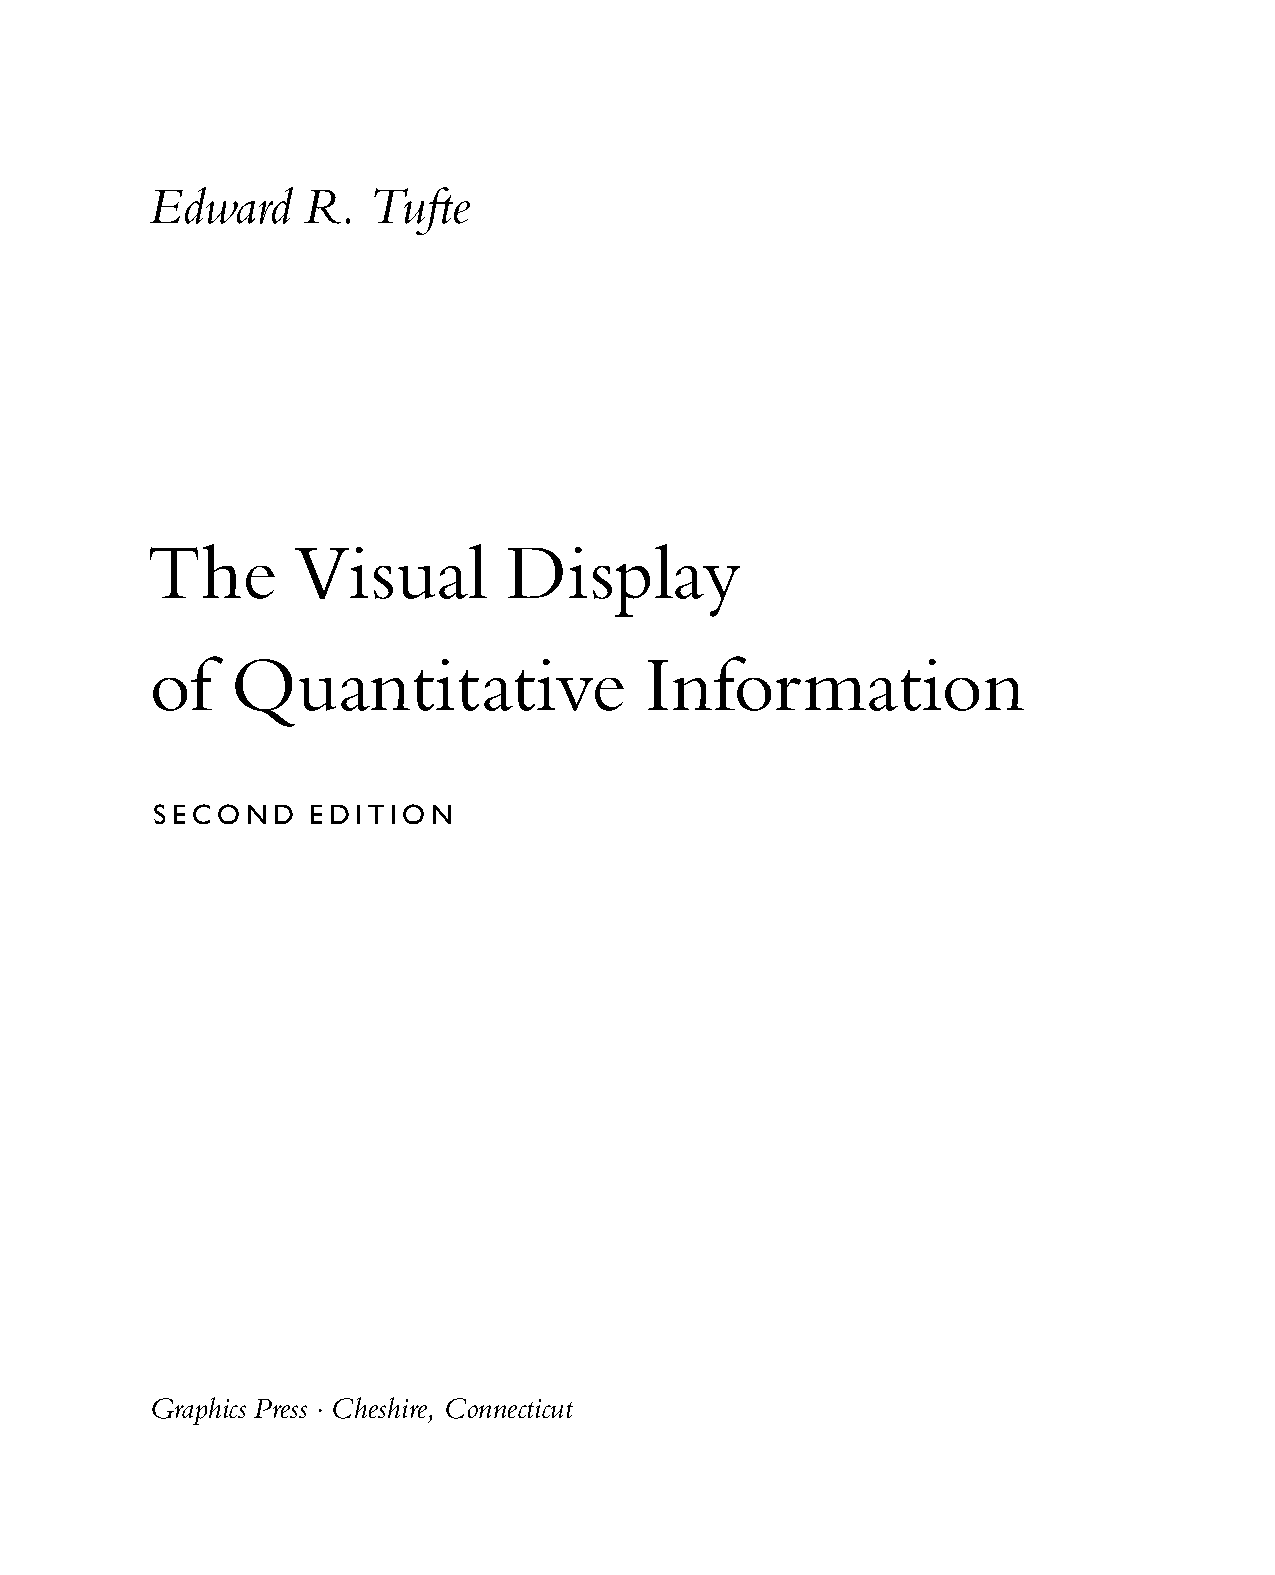
\includegraphics[width=0.45\linewidth]{vdqi-title.pdf}}
\hfill
\fbox{
\includegraphics[width=0.45\linewidth]{ei-title.pdf}}
\\\vspace{\baselineskip}
\fbox{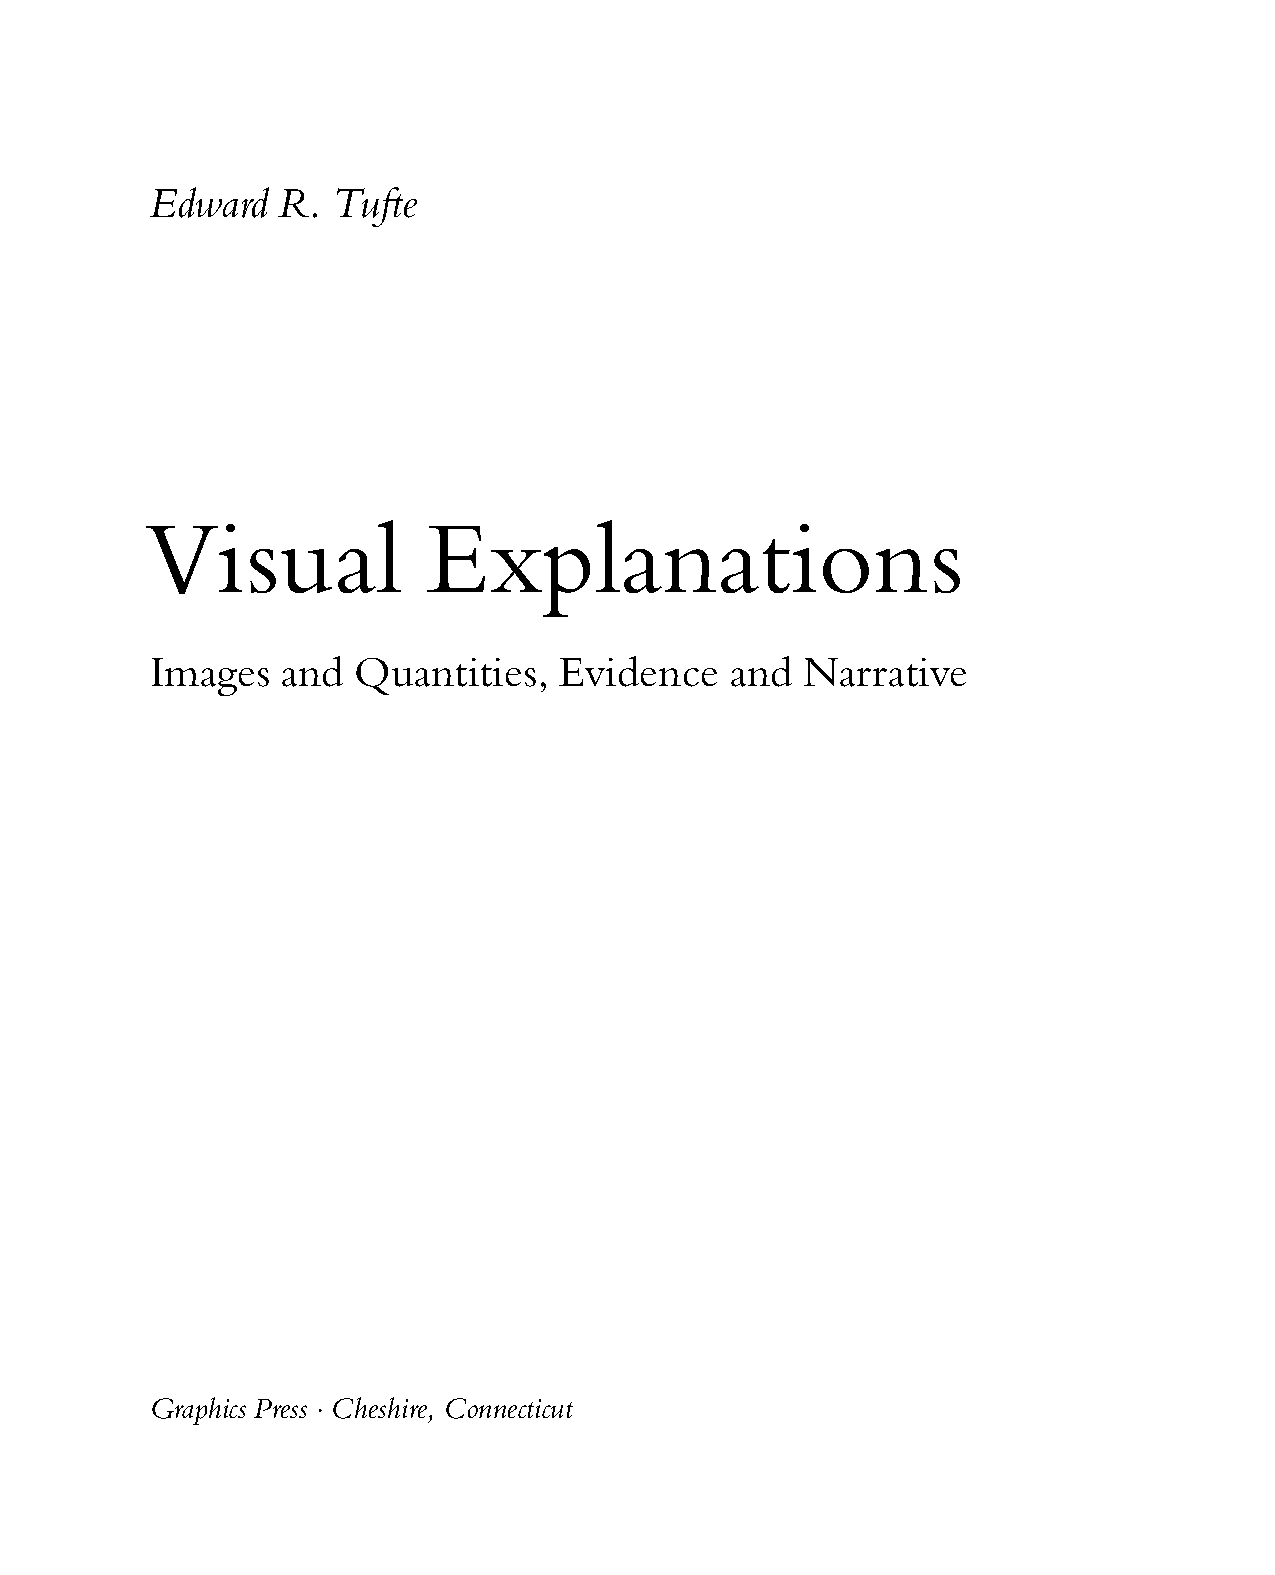
\includegraphics[width=0.45\linewidth]{ve-title.pdf}}
\hfill
\fbox{
\includegraphics[width=0.45\linewidth]{be-title.pdf}}
\end{figure*}

\newthought{The tables of contents} in Tufte's books give us our first
glimpse of the structure of the main matter.  \VDQI is split into two
parts, each containing some number of chapters.  His other three books only
contain chapters---they're not broken into parts.

\begin{figure*}[p]\index{table of contents}
\fbox{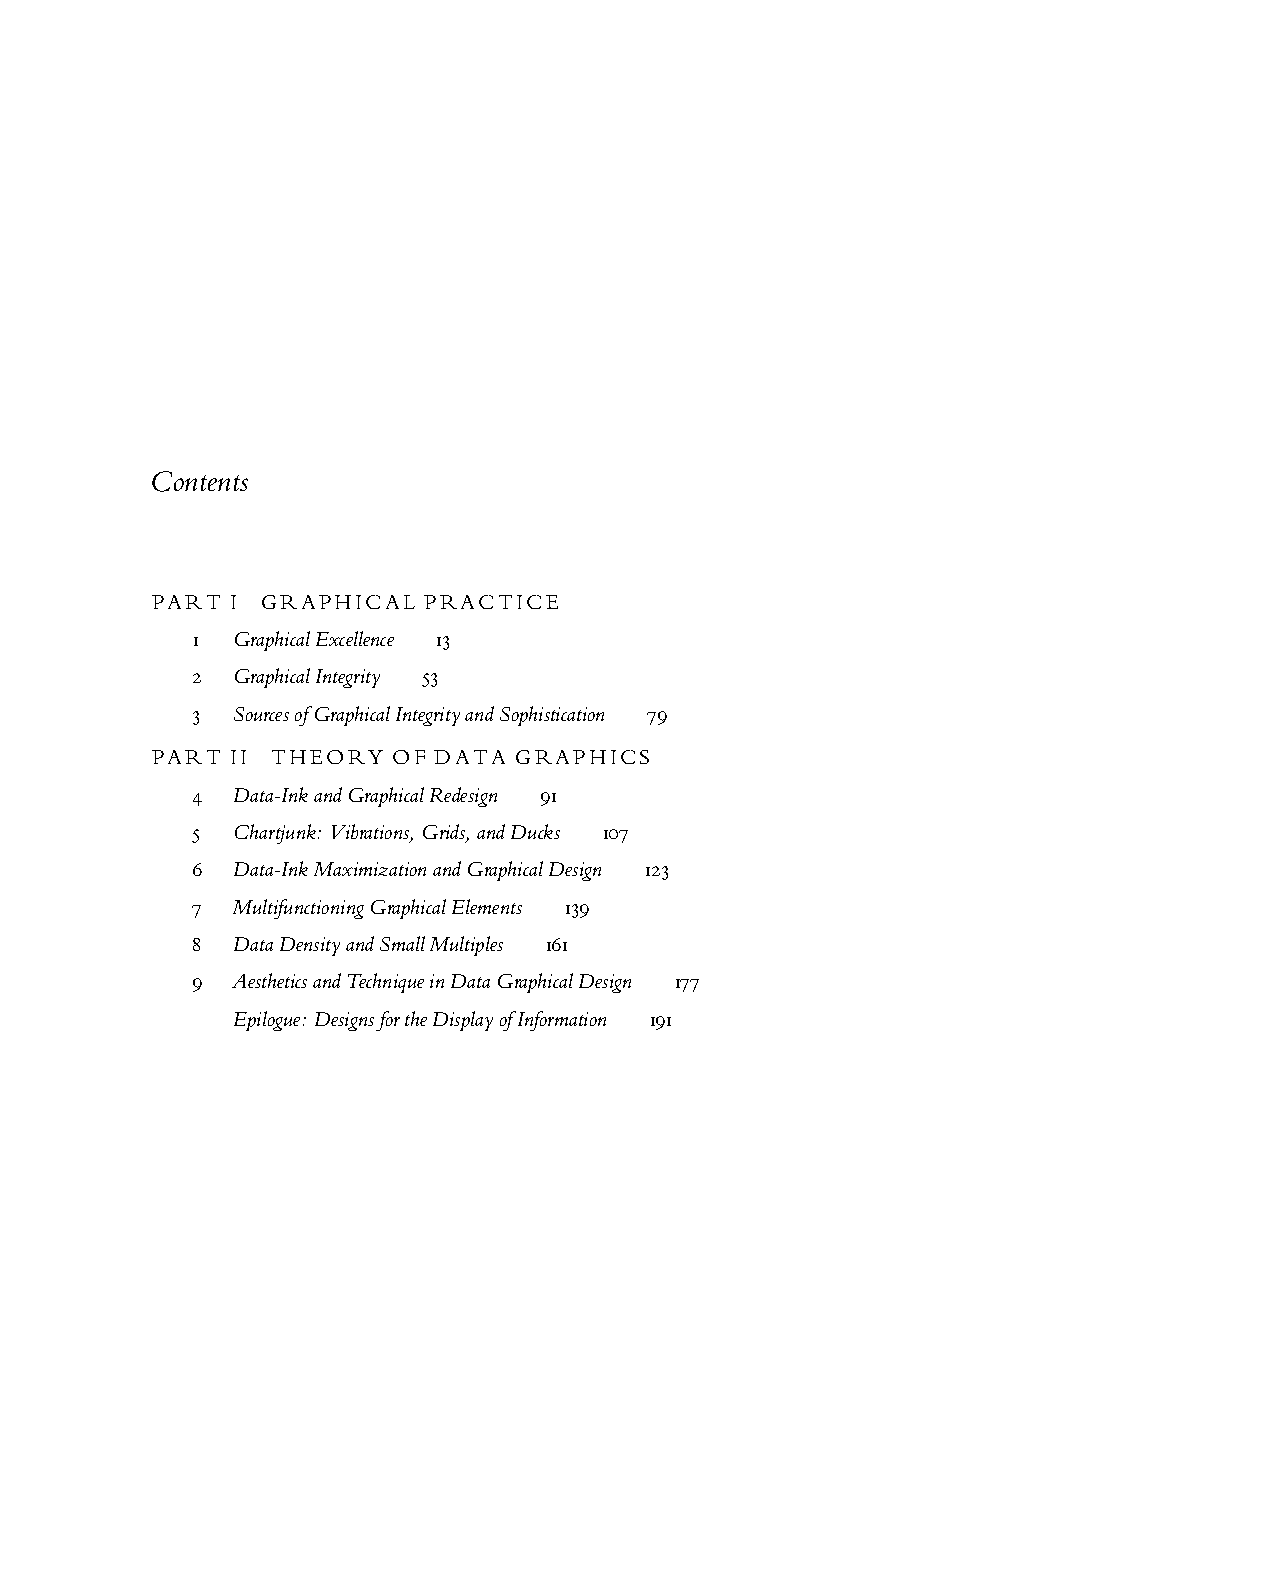
\includegraphics[width=0.45\linewidth]{vdqi-contents.pdf}}
\hfill
\fbox{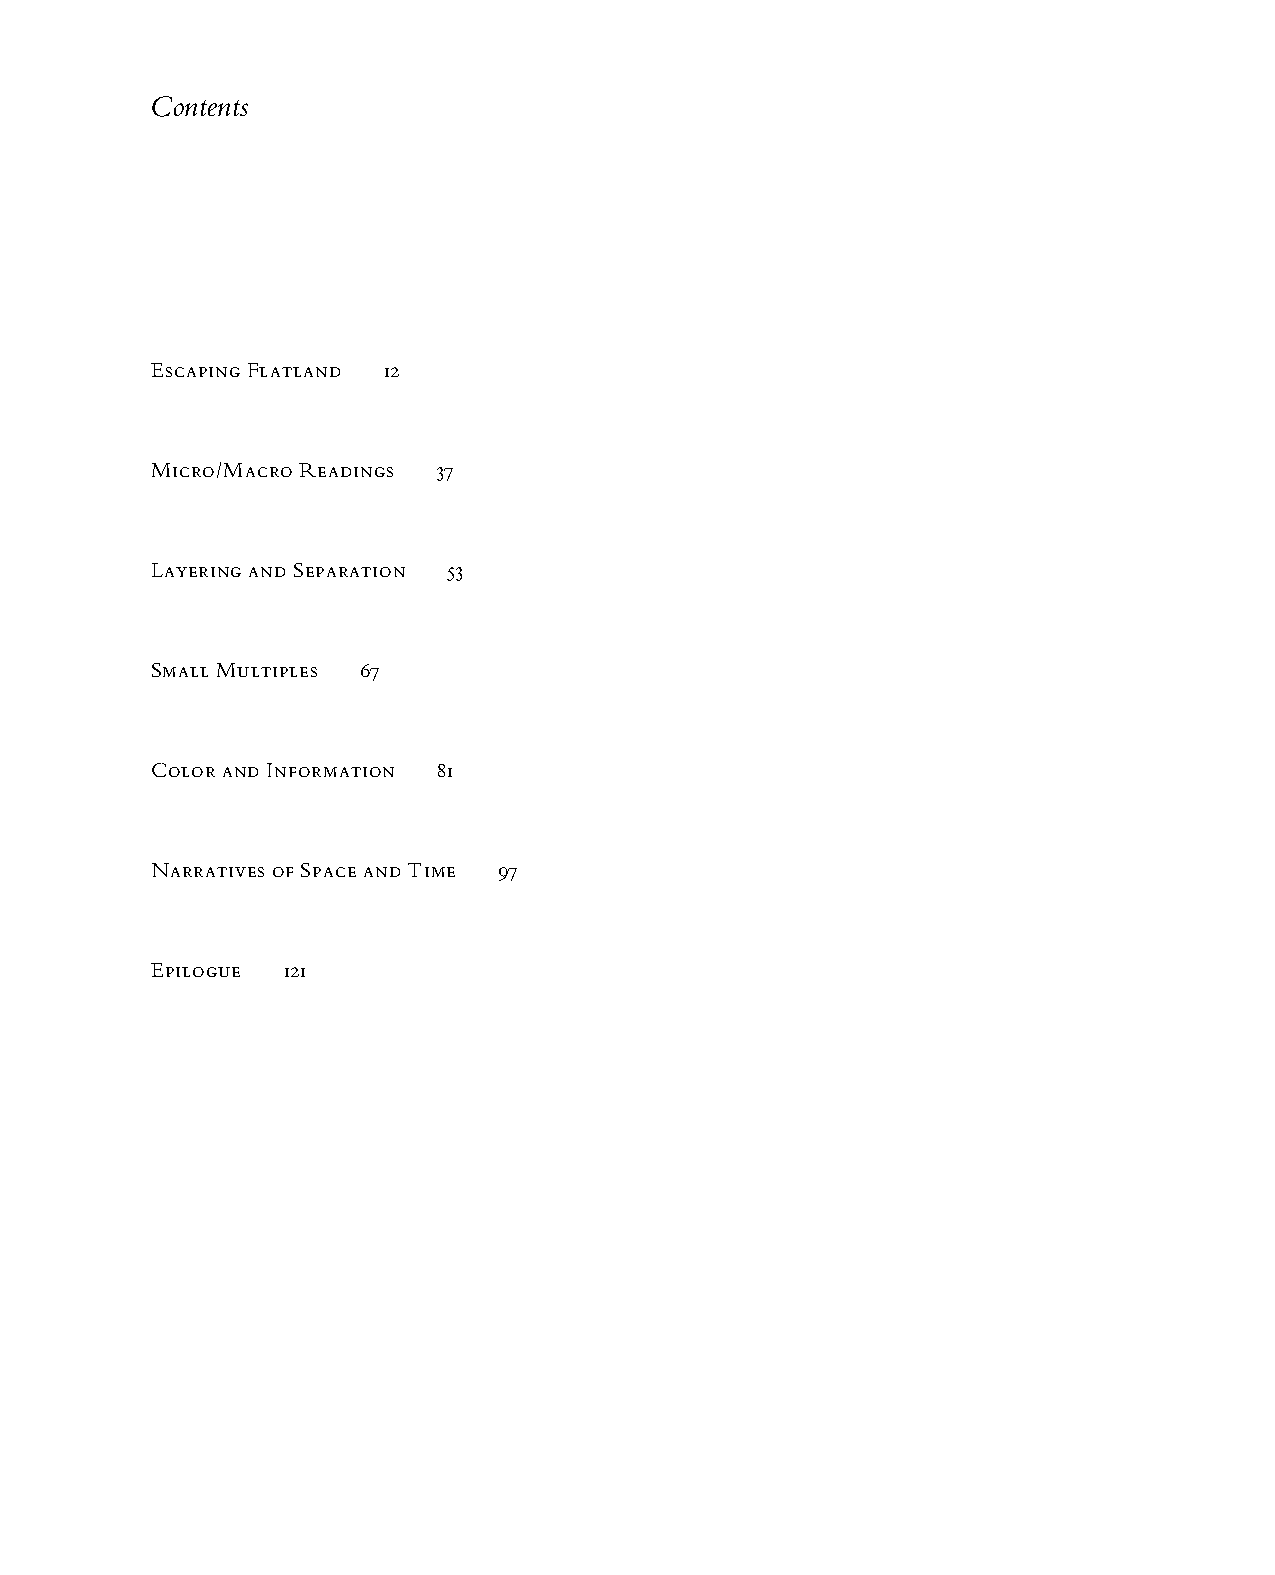
\includegraphics[width=0.45\linewidth]{ei-contents.pdf}}
\\\vspace{\baselineskip}
\fbox{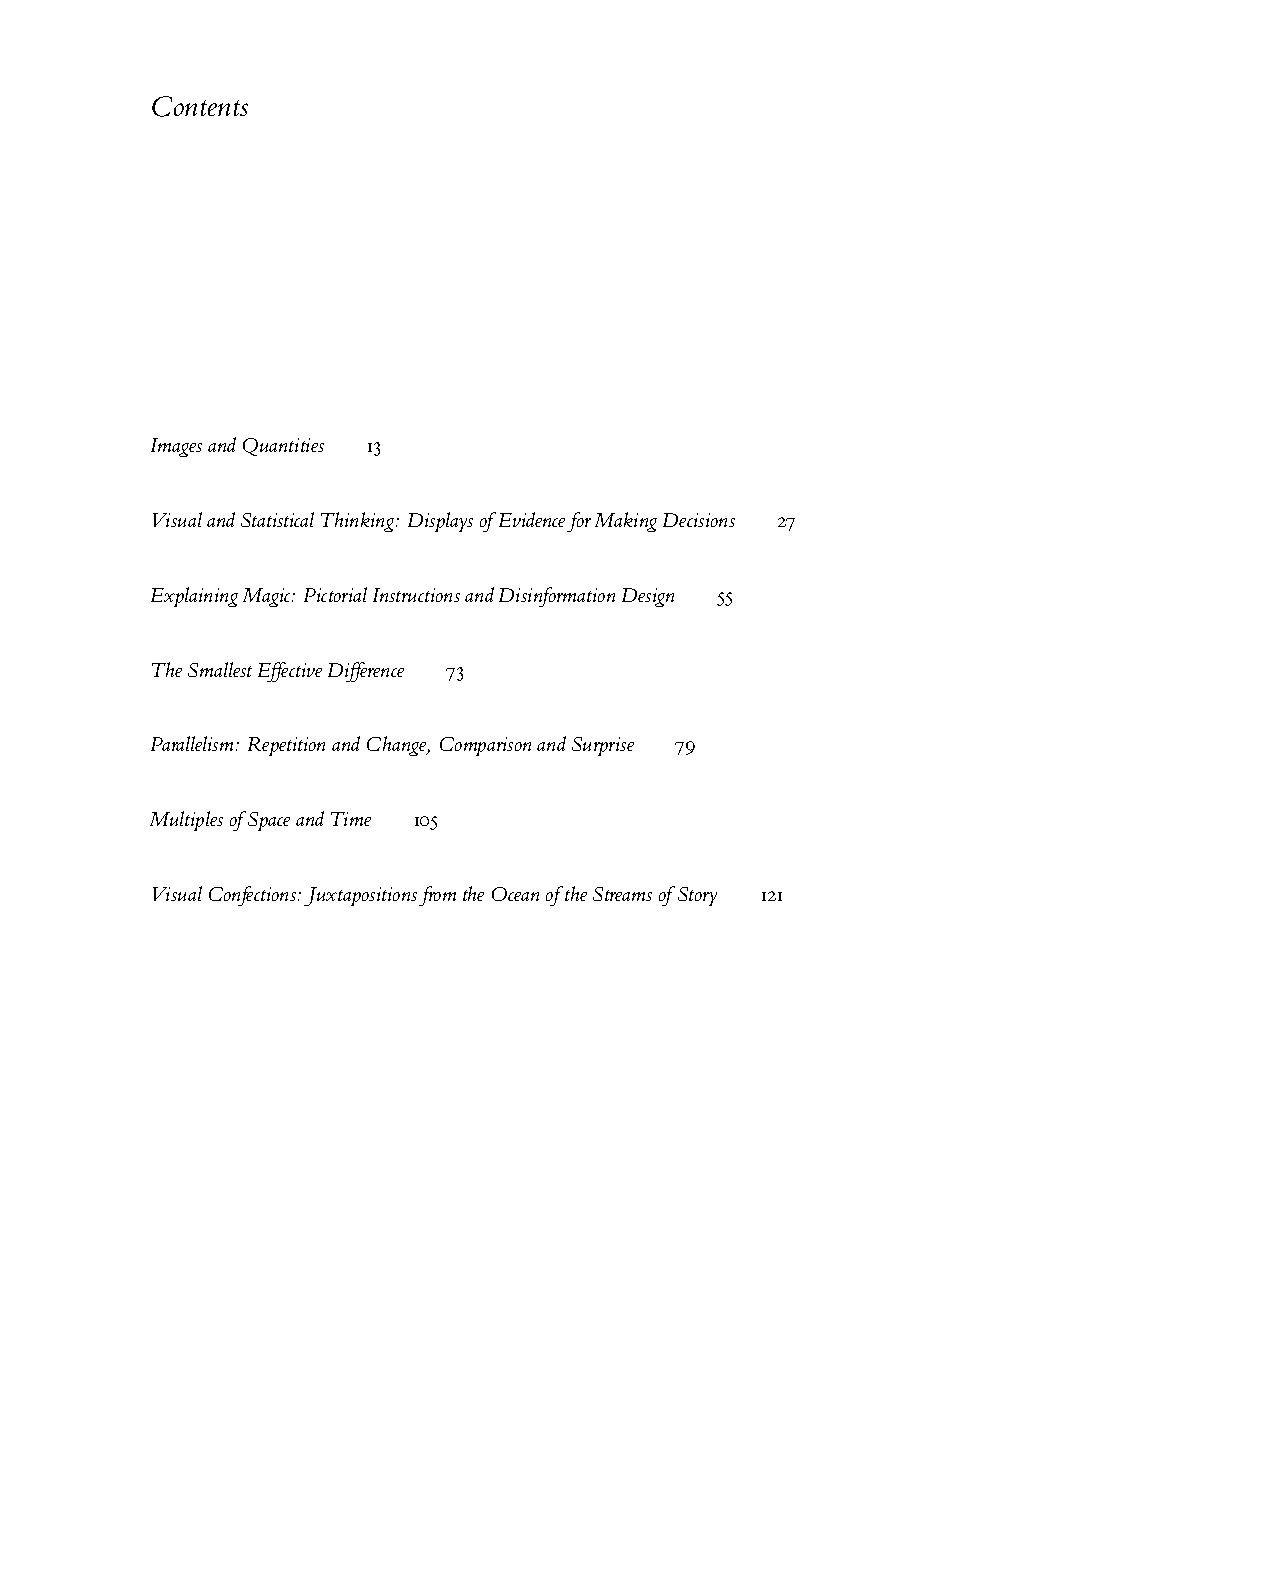
\includegraphics[width=0.45\linewidth]{ve-contents.pdf}}
\hfill
\fbox{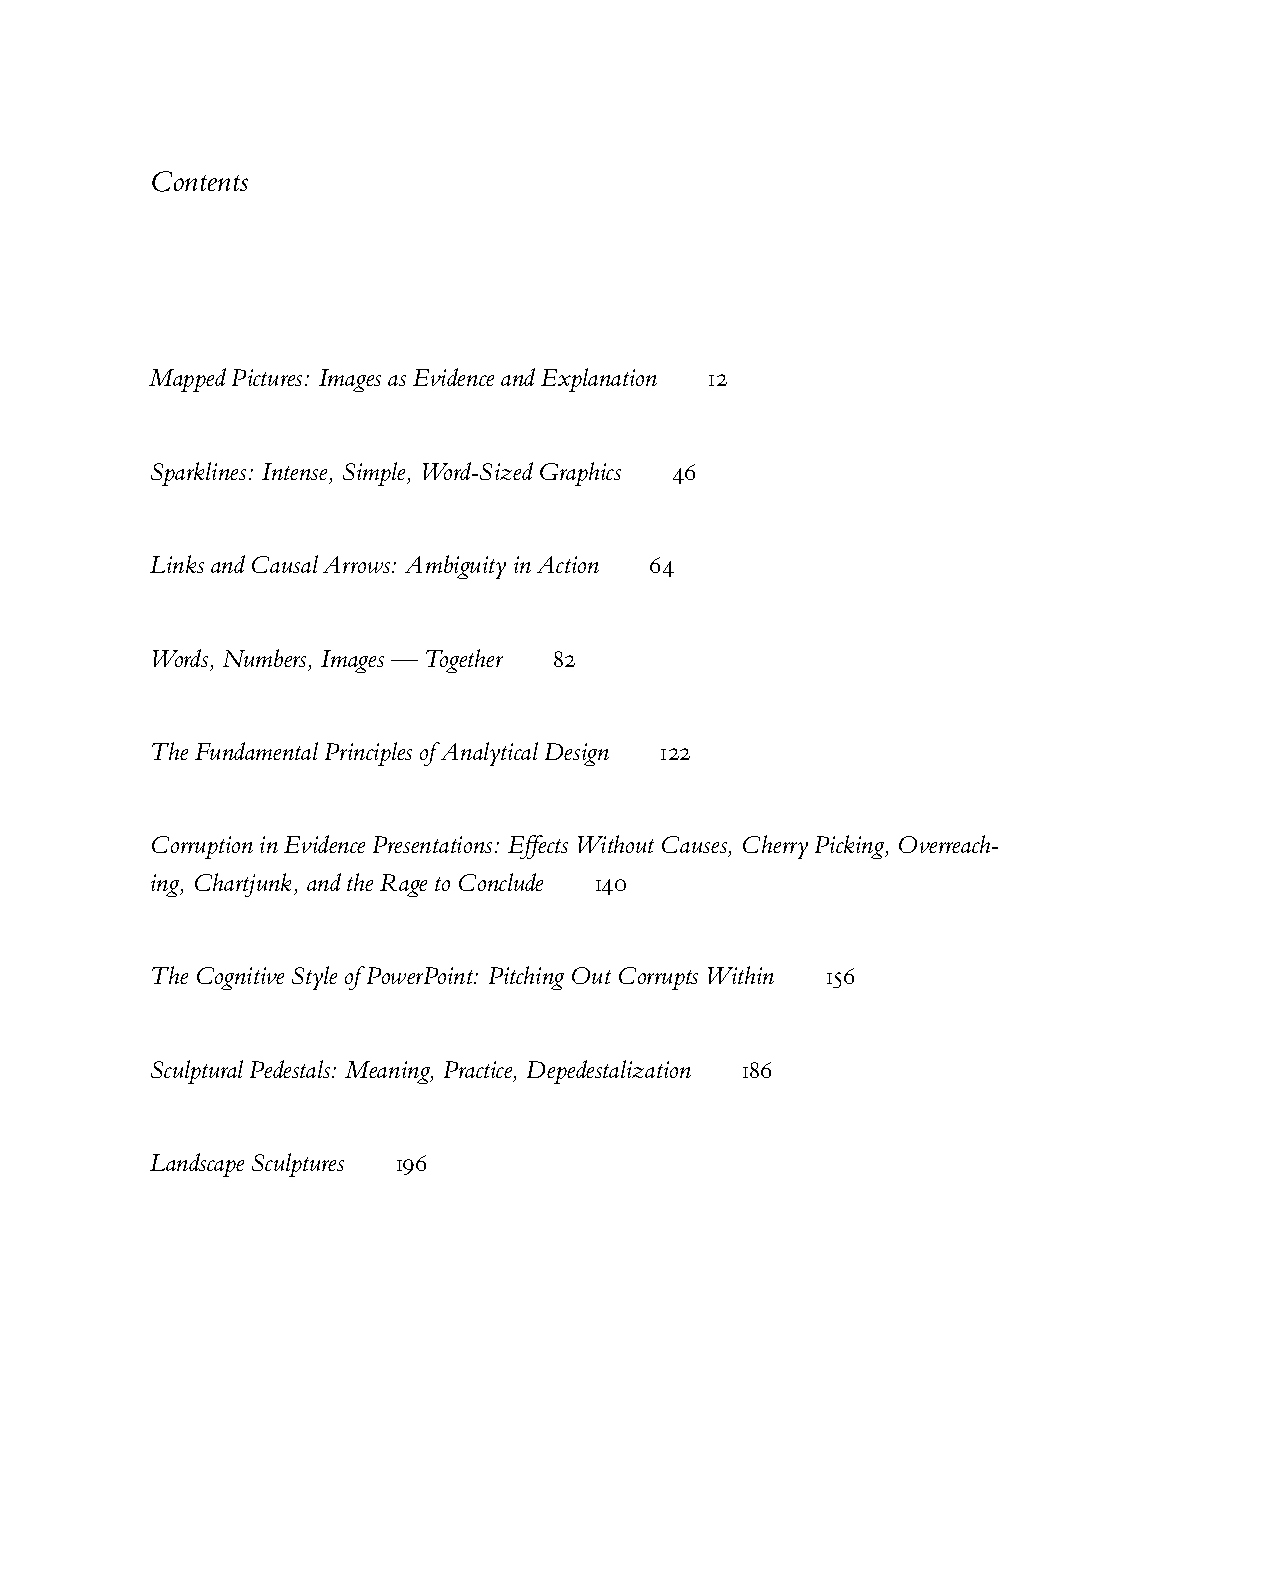
\includegraphics[width=0.45\linewidth]{be-contents.pdf}}
\end{figure*}


\section{Typefaces}\label{sec:typefaces1}\index{typefaces}
\index{fonts|see{typefaces}}

Tufte's books primarily use two typefaces: Bembo and Gill Sans.  Bembo is used
for the headings and body text, while Gill Sans is used for the title page and
opening epigraphs in \BE.

Since neither Bembo nor Gill Sans are available in default \LaTeX{}
installations, the \TL document classes default to using Palatino and
Helvetica, respectively.  In addition, the Bera Mono typeface is used for
\texttt{monospaced} type.

The following font sizes are defined by the \TL classes:

\begin{table}[h]\index{typefaces!sizes}
  \footnotesize%
  \begin{center}
    \begin{tabular}{lccl}
      \toprule
      \LaTeX{} size & Font size & Leading & Used for \\
      \midrule
      \verb+\tiny+         &  5 &  6 & sidenote numbers \\
      \verb+\scriptsize+   &  7 &  8 & \na \\
      \verb+\footnotesize+ &  8 & 10 & sidenotes, captions \\
      \verb+\small+        &  9 & 12 & quote, quotation, and verse environments \\
      \verb+\normalsize+   & 10 & 14 & body text \\
      \verb+\large+        & 11 & 15 & \textsc{b}-heads \\
      \verb+\Large+        & 12 & 16 & \textsc{a}-heads, \textsc{toc} entries, author, date \\
      \verb+\LARGE+        & 14 & 18 & handout title \\
      \verb+\huge+         & 20 & 30 & chapter heads \\
      \verb+\Huge+         & 24 & 36 & part titles \\
      \bottomrule
    \end{tabular}
  \end{center}
  \caption{A list of \LaTeX{} font sizes as defined by the \TL document classes.}
  \label{tab:font-sizes}
\end{table}

\section{Headings}\label{sec:headings1}\index{headings}

Tufte's books include the following heading levels: parts,
chapters,\sidenote{Parts and chapters are defined for the \texttt{tufte-book}
class only.}  sections, subsections, and paragraphs.  Not defined by default
are: sub-subsections and subparagraphs.

\begin{table}[h]
  \begin{center}
    \footnotesize%
    \begin{tabular}{lcr}
      \toprule
      Heading & Style & Size \\
      \midrule
      Part & roman & \measure{24}{36}{40} \\
      Chapter & italic & \measure{20}{30}{40} \\
      Section & italic & \measure{12}{16}{26} \\
      Subsection & italic & \measure{11}{15}{26} \\
      Paragraph & italic & 10/14 \\
      \bottomrule
    \end{tabular}
  \end{center}
  \caption{Heading styles used in \BE.}
  \label{tab:heading-styles}
\end{table}

\paragraph{Paragraph} Paragraph headings (as shown here) are introduced by
italicized text and separated from the main paragraph by a bit of space.

\section{Environments}

The following characteristics define the various environments:


\begin{table}[h]
  \begin{center}
    \footnotesize%
    \begin{tabular}{lcl}
      \toprule
      Environment & Font size & Notes \\
      \midrule
      Body text & \measure{10}{14}{26} & \\
      Block quote & \measure{9}{12}{24} & Block indent (left and right) by \unit[1]{pc} \\
      Sidenotes & \measure{8}{10}{12} & Sidenote number is set inline, followed by word space \\
      Captions & \measure{8}{10}{12} &  \\
      \bottomrule
    \end{tabular}
  \end{center}
  \caption{Environment styles used in \BE.}
  \label{tab:environment-styles}
\end{table}


\chapter[On the Use of the tufte-book Document Class]{On the Use of the \texttt{tufte-book} Document Class}
\label{ch:tufte-book}

The \TL document classes define a style similar to the
style Edward Tufte uses in his books and handouts.  Tufte's style is known
for its extensive use of sidenotes, tight integration of graphics with
text, and well-set typography.  This document aims to be at once a
demonstration of the features of the \TL document classes
and a style guide to their use.

\section{Page Layout}\label{sec:page-layout}
\subsection{Headings}\label{sec:headings}\index{headings}
This style provides \textsc{a}- and \textsc{b}-heads (that is,
\Verb|\section| and \Verb|\subsection|), demonstrated above.

If you need more than two levels of section headings, you'll have to define
them yourself at the moment; there are no pre-defined styles for anything below
a \Verb|\subsection|.  As Bringhurst points out in \textit{The Elements of
Typographic Style},\cite{Bringhurst2005} you should ``use as many levels of
headings as you need: no more, and no fewer.''

The \TL classes will emit an error if you try to use
\linebreak\Verb|\subsubsection| and smaller headings.

% let's start a new thought -- a new section
\newthought{In his later books},\cite{Tufte2006} Tufte
starts each section with a bit of vertical space, a non-indented paragraph,
and sets the first few words of the sentence in \textsc{small caps}.  To
accomplish this using this style, use the \doccmddef{newthought} command:
\begin{docspec}
  \doccmd{newthought}\{In his later books\}, Tufte starts\ldots
\end{docspec}


\section{Sidenotes}\label{sec:sidenotes}
One of the most prominent and distinctive features of this style is the
extensive use of sidenotes.  There is a wide margin to provide ample room
for sidenotes and small figures.  Any \doccmd{footnote}s will automatically
be converted to sidenotes.\footnote{This is a sidenote that was entered
using the \texttt{\textbackslash footnote} command.}  If you'd like to place ancillary
information in the margin without the sidenote mark (the superscript
number), you can use the \doccmd{marginnote} command.\marginnote{This is a
margin note.  Notice that there isn't a number preceding the note, and
there is no number in the main text where this note was written.}

The specification of the \doccmddef{sidenote} command is:
\begin{docspec}
  \doccmd{sidenote}[\docopt{number}][\docopt{offset}]\{\docarg{Sidenote text.}\}
\end{docspec}

Both the \docopt{number} and \docopt{offset} arguments are optional.  If you
provide a \docopt{number} argument, then that number will be used as the
sidenote number.  It will change of the number of the current sidenote only and
will not affect the numbering sequence of subsequent sidenotes.

Sometimes a sidenote may run over the top of other text or graphics in the
margin space.  If this happens, you can adjust the vertical position of the
sidenote by providing a dimension in the \docopt{offset} argument.  Some
examples of valid dimensions are:
\begin{docspec}
  \ttfamily 1.0in \qquad 2.54cm \qquad 254mm \qquad 6\Verb|\baselineskip|
\end{docspec}
If the dimension is positive it will push the sidenote down the page; if the
dimension is negative, it will move the sidenote up the page.

While both the \docopt{number} and \docopt{offset} arguments are optional, they
must be provided in order.  To adjust the vertical position of the sidenote
while leaving the sidenote number alone, use the following syntax:
\begin{docspec}
  \doccmd{sidenote}[][\docopt{offset}]\{\docarg{Sidenote text.}\}
\end{docspec}
The empty brackets tell the \Verb|\sidenote| command to use the default
sidenote number.

If you \emph{only} want to change the sidenote number, however, you may
completely omit the \docopt{offset} argument:
\begin{docspec}
  \doccmd{sidenote}[\docopt{number}]\{\docarg{Sidenote text.}\}
\end{docspec}

The \doccmddef{marginnote} command has a similar \docarg{offset} argument:
\begin{docspec}
  \doccmd{marginnote}[\docopt{offset}]\{\docarg{Margin note text.}\}
\end{docspec}

\section{References}
References are placed alongside their citations as sidenotes,
as well.  This can be accomplished using the normal \doccmddef{cite}
command.\sidenote{The first paragraph of this document includes a citation.}

The complete list of references may also be printed automatically by using
the \doccmddef{bibliography} command.  (See the end of this document for an
example.)  If you do not want to print a bibliographyn at the end of your
document, use the \doccmddef{nobibliography} command in its place.  

To enter multiple citations at one location,\cite[-3\baselineskip]{Tufte2006,Tufte1990} you can
provide a list of keys separated by commas and the same optional vertical
offset argument: \Verb|\cite{Tufte2006,Tufte1990}|.  
\begin{docspec}
  \doccmd{cite}[\docopt{offset}]\{\docarg{bibkey1,bibkey2,\ldots}\}
\end{docspec}

\section{Figures and Tables}\label{sec:figures-and-tables}
Images and graphics play an integral role in Tufte's work.
In addition to the standard \docenvdef{figure} and \docenvdef{tabular} environments,
this style provides special figure and table environments for full-width
floats.

Full page--width figures and tables may be placed in \docenvdef{figure*} or
\docenvdef{table*} environments.  To place figures or tables in the margin,
use the \docenvdef{marginfigure} or \docenvdef{margintable} environments as follows
(see figure~\ref{fig:marginfig}):

\begin{marginfigure}%
  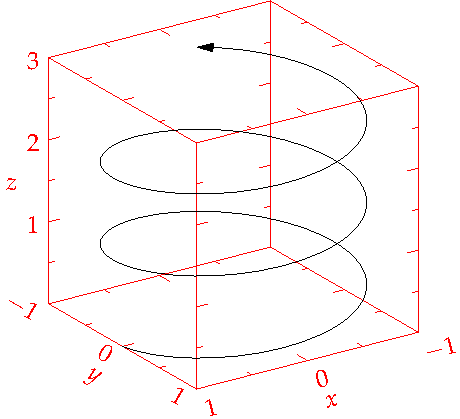
\includegraphics[width=\linewidth]{helix}
  \caption{This is a margin figure.  The helix is defined by 
    $x = \cos(2\pi z)$, $y = \sin(2\pi z)$, and $z = [0, 2.7]$.  The figure was
    drawn using Asymptote (\protect\url{http://asymptote.sf.net/}).}
  \label{fig:marginfig}
\end{marginfigure}

\begin{docspec}
\textbackslash begin\{marginfigure\}\\
  \qquad\textbackslash includegraphics\{helix\}\\
  \qquad\textbackslash caption\{This is a margin figure.\}\\
  \qquad\textbackslash label\{fig:marginfig\}\\
\textbackslash end\{marginfigure\}\\
\end{docspec}

The \docenv{marginfigure} and \docenv{margintable} environments accept an optional parameter \docopt{offset} that adjusts the vertical position of the figure or table.  See the ``\nameref{sec:sidenotes}'' section above for examples.  The specifications are:
\begin{docspec}
  \textbackslash{begin\{marginfigure\}[\docopt{offset}]}\\
  \qquad\ldots\\
  \textbackslash{end\{marginfigure\}}\\
  \mbox{}\\
  \textbackslash{begin\{margintable\}[\docopt{offset}]}\\
  \qquad\ldots\\
  \textbackslash{end\{margintable\}}\\
\end{docspec}

Figure~\ref{fig:fullfig} is an example of the \docenv{figure*}
environment and figure~\ref{fig:textfig} is an example of the normal
\docenv{figure} environment.

\begin{figure*}[h]
  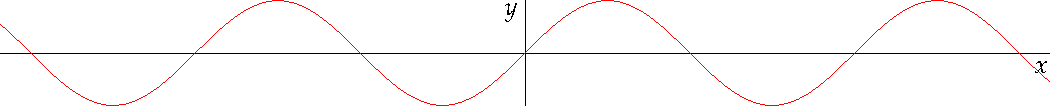
\includegraphics[width=\linewidth]{sine.pdf}%
  \caption{This graph shows $y = \sin x$ from about $x = [-10, 10]$.
  \emph{Notice that this figure takes up the full page width.}}%
  \label{fig:fullfig}%
\end{figure*}

\begin{figure}
  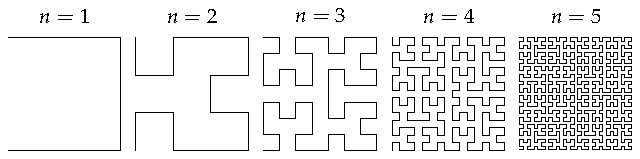
\includegraphics{hilbertcurves.pdf}
%  \checkparity This is an \pageparity\ page.%
  \caption[Hilbert curves of various degrees $n$.][6pt]{Hilbert curves of various degrees $n$. \emph{Notice that this figure only takes up the main textblock width.}}
  \label{fig:textfig}
  %\zsavepos{pos:textfig}
\end{figure}

As with sidenotes and marginnotes, a caption may sometimes require vertical
adjustment. The \doccmddef{caption} command now takes a second optional
argument that enables you to do this by providing a dimension \docopt{offset}.
You may specify the caption in any one of the following forms:
\begin{docspec}
  \doccmd{caption}\{\docarg{long caption}\}\\
  \doccmd{caption}[\docarg{short caption}]\{\docarg{long caption}\}\\
  \doccmd{caption}[][\docopt{offset}]\{\docarg{long caption}\}\\
  \doccmd{caption}[\docarg{short caption}][\docopt{offset}]%
                  \{\docarg{long caption}\}
\end{docspec}
A positive \docopt{offset} will push the caption down the page. The short
caption, if provided, is what appears in the list of figures/tables, otherwise
the ``long'' caption appears there. Note that although the arguments
\docopt{short caption} and \docopt{offset} are both optional, they must be
provided in order. Thus, to specify an \docopt{offset} without specifying a
\docopt{short caption}, you must include the first set of empty brackets
\Verb|[]|, which tell \doccmd{caption} to use the default ``long'' caption. As
an example, the caption to figure~\ref{fig:textfig} above was given in the form
\begin{docspec}
  \doccmd{caption}[Hilbert curves...][6pt]\{Hilbert curves...\}
\end{docspec}

Table~\ref{tab:normaltab} shows table created with the \docpkg{booktabs}
package.  Notice the lack of vertical rules---they serve only to clutter
the table's data.

\begin{table}[ht]
  \centering
  \fontfamily{ppl}\selectfont
  \begin{tabular}{ll}
    \toprule
    Margin & Length \\
    \midrule
    Paper width & \unit[8\nicefrac{1}{2}]{inches} \\
    Paper height & \unit[11]{inches} \\
    Textblock width & \unit[6\nicefrac{1}{2}]{inches} \\
    Textblock/sidenote gutter & \unit[\nicefrac{3}{8}]{inches} \\
    Sidenote width & \unit[2]{inches} \\
    \bottomrule
  \end{tabular}
  \caption{Here are the dimensions of the various margins used in the Tufte-handout class.}
  \label{tab:normaltab}
  %\zsavepos{pos:normaltab}
\end{table}

\newthought{Occasionally} \LaTeX{} will generate an error message:\label{err:too-many-floats}
\begin{docspec}
  Error: Too many unprocessed floats
\end{docspec}
\LaTeX{} tries to place floats in the best position on the page.  Until it's
finished composing the page, however, it won't know where those positions are.
If you have a lot of floats on a page (including sidenotes, margin notes,
figures, tables, etc.), \LaTeX{} may run out of ``slots'' to keep track of them
and will generate the above error.

\LaTeX{} initially allocates 18 slots for storing floats.  To work around this
limitation, the \TL document classes provide a \doccmddef{morefloats} command
that will reserve more slots.

The first time \doccmd{morefloats} is called, it allocates an additional 34
slots.  The second time \doccmd{morefloats} is called, it allocates another 26
slots.

The \doccmd{morefloats} command may only be used two times.  Calling it a
third time will generate an error message.  (This is because we can't safely
allocate many more floats or \LaTeX{} will run out of memory.)

If, after using the \doccmd{morefloats} command twice, you continue to get the
\texttt{Too many unprocessed floats} error, there are a couple things you can
do.

The \doccmddef{FloatBarrier} command will immediately process all the floats
before typesetting more material.  Since \doccmd{FloatBarrier} will start a new
paragraph, you should place this command at the beginning or end of a
paragraph.

The \doccmddef{clearpage} command will also process the floats before
continuing, but instead of starting a new paragraph, it will start a new page.

You can also try moving your floats around a bit: move a figure or table to the
next page or reduce the number of sidenotes.  (Each sidenote actually uses
\emph{two} slots.)

After the floats have placed, \LaTeX{} will mark those slots as unused so they
are available for the next page to be composed.

\section{Captions}
You may notice that the captions are sometimes misaligned.
Due to the way \LaTeX's float mechanism works, we can't know for sure where it
decided to put a float. Therefore, the \TL document classes provide commands to
override the caption position.

\paragraph{Vertical alignment} To override the vertical alignment, use the
\doccmd{setfloatalignment} command inside the float environment.  For
example:

\begin{fullwidth}
\begin{docspec}
  \textbackslash begin\{figure\}[btp]\\
  \qquad \textbackslash includegraphics\{sinewave\}\\
  \qquad \textbackslash caption\{This is an example of a sine wave.\}\\
  \qquad \textbackslash label\{fig:sinewave\}\\
  \qquad \hlred{\textbackslash setfloatalignment\{b\}\% forces caption to be bottom-aligned}\\
  \textbackslash end\{figure\}
\end{docspec}
\end{fullwidth}

\noindent The syntax of the \doccmddef{setfloatalignment} command is:

\begin{docspec}
  \doccmd{setfloatalignment}\{\docopt{pos}\}
\end{docspec}

\noindent where \docopt{pos} can be either \texttt{b} for bottom-aligned
captions, or \texttt{t} for top-aligned captions.

\paragraph{Horizontal alignment}\label{par:overriding-horizontal}
To override the horizontal alignment, use either the \doccmd{forceversofloat}
or the \doccmd{forcerectofloat} command inside of the float environment.  For
example:

\begin{fullwidth}
\begin{docspec}
  \textbackslash begin\{figure\}[btp]\\
  \qquad \textbackslash includegraphics\{sinewave\}\\
  \qquad \textbackslash caption\{This is an example of a sine wave.\}\\
  \qquad \textbackslash label\{fig:sinewave\}\\
  \qquad \hlred{\textbackslash forceversofloat\% forces caption to be set to the left of the float}\\
  \textbackslash end\{figure\}
\end{docspec}
\end{fullwidth}

The \doccmddef{forceversofloat} command causes the algorithm to assume the
float has been placed on a verso page---that is, a page on the left side of a
two-page spread.  Conversely, the \doccmddef{forcerectofloat} command causes
the algorithm to assume the float has been placed on a recto page---that is, a
page on the right side of a two-page spread.


\section{Full-width text blocks}

In addition to the new float types, there is a \docenvdef{fullwidth}
environment that stretches across the main text block and the sidenotes
area.

\begin{Verbatim}
\begin{fullwidth}
Lorem ipsum dolor sit amet...
\end{fullwidth}
\end{Verbatim}

\begin{fullwidth}
\small\itshape\lipsum[1]
\end{fullwidth}

\section{Typography}\label{sec:typography}

\subsection{Typefaces}\label{sec:typefaces}\index{typefaces}
If the Palatino, \textsf{Helvetica}, and \texttt{Bera Mono} typefaces are installed, this style
will use them automatically.  Otherwise, we'll fall back on the Computer Modern
typefaces.

\subsection{Letterspacing}\label{sec:letterspacing}
This document class includes two new commands and some improvements on
existing commands for letterspacing.

When setting strings of \allcaps{ALL CAPS} or \smallcaps{small caps}, the
letter\-spacing---that is, the spacing between the letters---should be
increased slightly.\cite[][p.32]{Bringhurst2005} The \doccmddef{allcaps} command has proper letterspacing for
strings of \allcaps{FULL CAPITAL LETTERS}, and the \doccmddef{smallcaps} command
has letterspacing for \smallcaps{small capital letters}.  These commands
will also automatically convert the case of the text to upper- or
lowercase, respectively.

The \doccmddef{textsc} command has also been redefined to include
letterspacing.  The case of the \doccmd{textsc} argument is left as is,
however.  This allows one to use both uppercase and lowercase letters:
\textsc{The Initial Letters Of The Words In This Sentence Are Capitalized.}



\section{Document Class Options}\label{sec:options}

\index{class options|(}
The \doccls{tufte-book} class is based on the \LaTeX\ \doccls{book}
document class.  Therefore, you can pass any of the typical book
options.  There are a few options that are specific to the
\doccls{tufte-book} document class, however.

The \docclsoptdef{a4paper} option will set the paper size to \smallcaps{A4} instead of
the default \smallcaps{US} letter size.

The \docclsoptdef{sfsidenotes} option will set the sidenotes and title block in a 
\textsf{sans serif} typeface instead of the default roman.

The \docclsoptdef{twoside} option will modify the running heads so that the page
number is printed on the outside edge (as opposed to always printing the page
number on the right-side edge in \docclsoptdef{oneside} mode).  

The \docclsoptdef{symmetric} option typesets the sidenotes on the outside edge of
the page.  This is how books are traditionally printed, but is contrary to
Tufte's book design which sets the sidenotes on the right side of the page.
This option implicitly sets the \docclsopt{twoside} option.

The \docclsoptdef{justified} option sets all the text fully justified (flush left
and right).  The default is to set the text ragged right.  
The body text of Tufte's books are set ragged right.  This prevents
needless hyphenation and makes it easier to read the text in the slightly
narrower column.

The \docclsoptdef{bidi} option loads the \docpkg{bidi} package which is used with
\tXeLaTeX\ to typeset bi-directional text.  Since the \docpkg{bidi}
package needs to be loaded before the sidenotes and cite commands are defined,
it can't be loaded in the document preamble.

The \docclsoptdef{debug} option causes the \TL classes to output debug
information to the log file which is useful in troubleshooting bugs.  It will
also cause the graphics to be replaced by outlines.

The \docclsoptdef{nofonts} option prevents the \TL classes from
automatically loading the Palatino and Helvetica typefaces.  You should use
this option if you wish to load your own fonts.  If you're using \tXeLaTeX, this
option is implied (\ie, the Palatino and Helvetica fonts aren't loaded if you
use \tXeLaTeX).  

The \docclsoptdef{nols} option inhibits the letterspacing code.  The \TL\
classes try to load the appropriate letterspacing package (either pdf\TeX's
\docpkg{letterspace} package or the \docpkg{soul} package).  If you're using
\tXeLaTeX\ with \docpkg{fontenc}, however, you should configure your own
letterspacing.  

The \docclsoptdef{notitlepage} option causes \doccmd{maketitle} to generate a title
block instead of a title page.  The \doccls{book} class defaults to a title
page and the \doccls{handout} class defaults to the title block.  There is an
analogous \docclsoptdef{titlepage} option that forces \doccmd{maketitle} to
generate a full title page instead of the title block.

The \docclsoptdef{notoc} option suppresses \TL's custom table of contents
(\textsc{toc}) design.  The current \textsc{toc} design only shows unnumbered
chapter titles; it doesn't show sections or subsections.  The \docclsopt{notoc}
option will revert to \LaTeX's \textsc{toc} design.

The \docclsoptdef{nohyper} option prevents the \docpkg{hyperref} package from
being loaded.  The default is to load the \docpkg{hyperref} package and use the
\doccmd{title} and \doccmd{author} contents as metadata for the generated
\textsc{pdf}.

\index{class options|)}



\chapter[Customizing Tufte-LaTeX]{Customizing \TL}
\label{ch:customizing}

The \TL document classes are designed to closely emulate Tufte's book
design by default.  However, each document is different and you may encounter
situations where the default settings are insufficient.  This chapter explores
many of the ways you can adjust the \TL document classes to better fit
your needs.

\section{File Hooks}
\label{sec:filehooks}

\index{file hooks|(}
If you create many documents using the \TL classes, it's easier to
store your customizations in a separate file instead of copying them into the
preamble of each document.  The \TL classes provide three file hooks:
\docfilehook{tufte-common-local.tex}{common}, \docfilehook{tufte-book-local.tex}{book}, and
\docfilehook{tufte-handout-local.tex}{handout}.\sloppy

\begin{description}
  \item[\docfilehook{tufte-common-local.tex}{common}]
    If this file exists, it will be loaded by all of the \TL document
    classes just prior to any document-class-specific code.  If your
    customizations or code should be included in both the book and handout
    classes, use this file hook.
  \item[\docfilehook{tufte-book-local.tex}{book}] 
    If this file exists, it will be loaded after all of the common and
    book-specific code has been read.  If your customizations apply only to the
    book class, use this file hook.
  \item[\docfilehook{tufte-common-handout.tex}{handout}] 
    If this file exists, it will be loaded after all of the common and
    handout-specific code has been read.  If your customizations apply only to
    the handout class, use this file hook.
\end{description}

\index{file hooks|)}

\section{Numbered Section Headings}
\label{sec:numbered-sections}
\index{headings!numbered}

While Tufte dispenses with numbered headings in his books, if you require them,
they can be anabled by changing the value of the \doccounter{secnumdepth}
counter.  From the table below, select the heading level at which numbering
should stop and set the \doccounter{secnumdepth} counter to that value.  For
example, if you want parts and chapters numbered, but don't want numbering for
sections or subsections, use the command:
\begin{docspec}
  \doccmd{setcounter}\{secnumdepth\}\{0\}
\end{docspec}

The default \doccounter{secnumdepth} for the \TL document classes is $-1$.

\begin{table}
  \footnotesize
  \begin{center}
    \begin{tabular}{lr}
      \toprule
      Heading level & Value \\
      \midrule
      Part (in \doccls{tufte-book}) & $-1$ \\
      Part (in \doccls{tufte-handout}) & $0$ \\
      Chapter (only in \doccls{tufte-book}) & $0$ \\
      Section & $1$ \\
      Subsection & $2$ \\
      Subsubsection & $3$ \\
      Paragraph & $4$ \\
      Subparagraph & $5$ \\
      \bottomrule
    \end{tabular}
  \end{center}
  \caption{Heading levels used with the \texttt{secnumdepth} counter.}
\end{table}

\section{Changing the Paper Size}
\label{sec:paper-size}

The \TL classes currently only provide three paper sizes: \textsc{a4},
\textsc{b5}, and \textsc{us} letter.  To specify a different paper size (and/or
margins), use the \doccmd[geometry]{geometrysetup} command in the preamble of your
document (or one of the file hooks).  The full documentation of the
\doccmd{geometrysetup} command may be found in the \docpkg{geometry} package
documentation.\cite[-1em][p.33]{pkg-geometry}


\section{Customizing Marginal Material}
\label{sec:marginal-material}

Marginal material includes sidenotes, citations, margin notes, and captions.
Normally, the justification of the marginal material follows the justification
of the body text.  If you specify the \docclsopt{justified} document class
option, all of the margin material will be fully justified as well.  If you
don't specify the \docclsopt{justified} option, then the marginal material will
be set ragged right.

You can set the justification of the marginal material separately from the body
text using the following document class options: \docclsopt{sidenote},
\docclsopt{marginnote}, \docclsopt{caption}, \docclsopt{citation}, and
\docclsopt{marginals}.  Each option refers to its obviously corresponding
marginal material type.  The \docclsopt{marginals} option simultaneously sets
the justification on all four marginal material types.

Each of the document class options takes one of five justification types:
\begin{description}
  \item[\docclsopt{justified}] Fully justifies the text (sets it flush left and
    right).
  \item[\docclsopt{raggedleft}] Sets the text ragged left, regardless of which
    page it falls on.
  \item[\docclsopt{raggedright}] Sets the text ragged right, regardless of
    which page it falls on.
  \item[\doccls{raggedouter}] Sets the text ragged left if it falls on the
    left-hand (verso) page of the spread and otherwise sets it ragged right.
    This is useful in conjunction with the \docclsopt{symmetric} document class
    option.
  \item[\docclsopt{auto}] If the \docclsopt{justified} document class option
    was specified, then set the text fully justified; otherwise the text is set
    ragged right.  This is the default justification option if one is not
    explicitly specified.
\end{description}

\noindent For example, 
\begin{docspec}
  \doccmdnoindex{documentclass}[symmetric,justified,marginals=raggedouter]\{tufte-book\}
\end{docspec}
will set the body text of the document to be fully justified and all of the
margin material (sidenotes, margin notes, captions, and citations) to be flush
against the body text with ragged outer edges.

\newthought{The font and style} of the marginal material may also be modified using the following commands:

\begin{docspec}
  \doccmd{setsidenotefont}\{\docopt{font commands}\}\\
  \doccmd{setcaptionfont}\{\docopt{font commands}\}\\
  \doccmd{setmarginnotefont}\{\docopt{font commands}\}\\
  \doccmd{setcitationfont}\{\docopt{font commands}\}
\end{docspec}

The \doccmddef{setsidenotefont} sets the font and style for sidenotes, the
\doccmddef{setcaptionfont} for captions, the \doccmddef{setmarginnotefont} for
margin notes, and the \doccmddef{setcitationfont} for citations.  The
\docopt{font commands} can contain font size changes (e.g.,
\doccmdnoindex{footnotesize}, \doccmdnoindex{Huge}, etc.), font style changes (e.g.,
\doccmdnoindex{sffamily}, \doccmdnoindex{ttfamily}, \doccmdnoindex{itshape}, etc.), color changes (e.g.,
\doccmdnoindex{color}\texttt{\{blue\}}), and many other adjustments.

If, for example, you wanted the captions to be set in italic sans serif, you could use:
\begin{docspec}
  \doccmd{setcaptionfont}\{\doccmdnoindex{itshape}\doccmdnoindex{sffamily}\}
\end{docspec}

\chapter{Compatibility Issues}
\label{ch:compatibility}

When switching an existing document from one document class to a \TL document class, a few changes to the document may have to be made.

\section{Converting from \doccls{article} to \doccls{tufte-handout}}

The following \doccls{article} class options are unsupported: \docclsopt{10pt}, \docclsopt{11pt}, \docclsopt{12pt}, \docclsopt{a5paper}, \docclsopt{b5paper}, \docclsopt{executivepaper}, \docclsopt{legalpaper}, \docclsopt{landscape}, \docclsopt{onecolumn}, and \doccls{twocolumn}.

The following headings are not supported: \doccmd{subsubsection} and \doccmd{subparagraph}.

\section{Converting from \doccls{book} to \doccls{tufte-book}}

The following \doccls{report} class options are unsupported: \docclsopt{10pt}, \docclsopt{11pt}, \docclsopt{12pt}, \docclsopt{a5paper}, \docclsopt{b5paper}, \docclsopt{executivepaper}, \docclsopt{legalpaper}, \docclsopt{landscape}, \docclsopt{onecolumn}, and \doccls{twocolumn}.

The following headings are not supported: \doccmd{subsubsection} and \doccmd{subparagraph}.



\chapter{Troubleshooting and Support}
\label{ch:troubleshooting}

\section{\TL Website}\label{sec:website}
The website for the \TL packages is located at
\url{http://code.google.com/p/tufte-latex/}.  On our website, you'll find
links to our \smallcaps{svn} repository, mailing lists, bug tracker, and documentation.

\section{\TL Mailing Lists}\label{sec:mailing-lists}
There are two mailing lists for the \TL project:

\paragraph{Discussion list}
The \texttt{tufte-latex} discussion list is for asking questions, getting
assistance with problems, and help with troubleshooting.  Release announcements
are also posted to this list.  You can subscribe to the \texttt{tufte-latex}
discussion list at \url{http://groups.google.com/group/tufte-latex}.

\paragraph{Commits list}
The \texttt{tufte-latex-commits} list is a read-only mailing list.  A message
is sent to the list any time the \TL code has been updated.  If you'd like to
keep up with the latest code developments, you may subscribe to this list.  You
can subscribe to the \texttt{tufte-latex-commits} mailing list at
\url{http://groups.google.com/group/tufte-latex-commits}.

\section{Getting Help}\label{sec:getting-help}
If you've encountered a problem with one of the \TL document classes, have a
question, or would like to report a bug, please send an email to our
mailing list or visit our website.

To help us troubleshoot the problem more quickly, please try to compile your
document using the \docclsopt{debug} class option and send the generated
\texttt{.log} file to the mailing list with a brief description of the problem.



\section{Errors, Warnings, and Informational Messages}\label{sec:tl-messages}
The following is a list of all of the errors, warnings, and other messages generated by the \TL classes and a brief description of their meanings.
\index{error messages}\index{warning messages}\index{debug messages}

% Errors
\docmsg{Error: \doccmd{subparagraph} is undefined by this class.}{%
The \doccmd{subparagraph} command is not defined in the \TL document classes.
If you'd like to use the \doccmd{subparagraph} command, you'll need to redefine
it yourself.  See the ``Headings'' section on page~\pageref{sec:headings} for a
description of the heading styles availaboe in the \TL document classes.}

\docmsg{Error: \doccmd{subsubsection} is undefined by this class.}{%
The \doccmd{subsubsection} command is not defined in the \TL document classes.
If you'd like to use the \doccmd{subsubsection} command, you'll need to
redefine it yourself.  See the ``Headings'' section on
page~\pageref{sec:headings} for a description of the heading styles availaboe
in the \TL document classes.}

\docmsg{Error: You may only call \doccmd{morefloats} twice. See the\par\noindent\ \ \ \ \ \ \ \ Tufte-LaTeX documentation for other workarounds.}{%
\LaTeX{} allocates 18 slots for storing floats.  The first time
\doccmd{morefloats} is called, it allocates an additional 34 slots.  The second
time \doccmd{morefloats} is called, it allocates another 26 slots.

The \doccmd{morefloats} command may only be called two times.  Calling it a
third time will generate this error message.  See
page~\pageref{err:too-many-floats} for more information.}

% Warnings
\docmsg{Warning: Option `\docopt{class option}' is not supported -{}- ignoring option.}{%
This warning appears when you've tried to use \docopt{class option} with a \TL
document class, but \docopt{class option} isn't supported by the \TL document
class.  In this situation, \docopt{class option} is ignored.}

% Info / Debug messages
\docmsg{Info: The `\docclsopt{symmetric}' option implies `\docclsopt{twoside}'}{%
You specified the \docclsopt{symmetric} document class option.  This option automatically forces the \docclsopt{twoside} option as well.  See page~\pageref{clsopt:symmetric} for more information on the \docclsopt{symmetric} class option.}


\section{Package Dependencies}\label{sec:dependencies}
The following is a list of packages that the \TL document
classes rely upon.  Packages marked with an asterisk are optional.
\begin{multicols}{2}
\begin{itemize}
  \item xifthen
  \item ifpdf*
  \item ifxetex*
  \item hyperref
  \item geometry
  \item ragged2e
  \item chngpage \emph{or} changepage
  \item paralist
  \item textcase
  \item soul*
  \item letterspace*
  \item setspace
  \item natbib \emph{and} bibentry
  \item optparams
  \item placeins
  \item mathpazo*
  \item helvet*
  \item fontenc
  \item beramono*
  \item fancyhdr
  \item xcolor
  \item textcomp
  \item titlesec
  \item titletoc
\end{itemize}
\end{multicols}




%%
% The back matter contains appendices, bibliographies, indices, glossaries, etc.







% \bibliography{sample-handout}
% \bibliographystyle{plainnat}
\printindex

\end{document}
